\documentclass[a4paper, 12pt, openany]{book} %chose the paper size and font size. Openany ensures that all all chapters and similar may begin at any page, not only odd pages. For the introductory pages and appendices we want openany, but for chapter pages in the main content we want chapters to begin only on odd pages (right hand side). The book class ensures that the margins are automatically adjusted such that left hand pages are slightly moved to the left and vice versa at the right, which makes the thesis very readable and good looking when printed in


\usepackage[utf8]{inputenc} %to manage special characters
\usepackage[T1]{fontenc} %to manage special characters
\usepackage[Bjarne]{fncychap} %fancy chapter style (many more available, like Sonny or Lenny etc.)
\usepackage{fancyhdr} %to customize the headers
\usepackage[lmargin=1.5in, rmargin=1in, tmargin=1in, bmargin=1in]{geometry} %sets the margins for the pages
\setcounter{tocdepth}{2} %table of contents number depth for subsections (2 = x.x.x)
\setcounter{secnumdepth}{4} %numbering depth for headers for subsections in the text(4 = x.x.x.x)
\usepackage{url} %to include urls
\usepackage{listings} %include this if you want to include code in the thesis
\usepackage{amsmath,amssymb} %mathematical package
\usepackage{siunitx} %includes SI-units
\usepackage[bf]{caption} %makes float captions bold
\usepackage{array, booktabs} %to make better tables
\usepackage{graphicx} %to include graphics
\usepackage{float} %to include floats
\usepackage[export]{adjustbox} %to adjust floats
\usepackage{subfig} %to include subfigures
\usepackage{chngcntr} %will make it possible to change the counter for tables, figures etc. such as below
\counterwithin{figure}{chapter} %change counter for figures within sections (also possible to choose for each chapter
\counterwithin{table}{chapter} %change counter for tables within sections
\usepackage{color, xcolor} %edit e.g. text colors

% \usepackage[backend = biber,
%             style = numeric,
%             date = long,     % Long: 24th Mar. 1997 | Short: 24/03/1997
%             sorting = none,
%             maxcitenames = 3,   % max names to include before et. al.
%             ]{biblatex} %customize the look of your citations and bibliography
\usepackage{natbib}
\bibliographystyle{abbrvnat}
\setcitestyle{authoryear}
% \addbibresource{references.bib} %declare the bibliography resource
\usepackage{comment} %to be able to comment out sections in the .tex files
\usepackage{afterpage} %to customize page commands such as below
\newcommand\myemptypage{
    \null
    \thispagestyle{empty}
    \addtocounter{page}{-1}
    \newpage
    } %sets new page command to insert an empty page without adding to the page counter or having a page number
\newcommand\taffo{{\em Taffo}}
\newcommand\floatsmith{{\em FloatSmith}}

\usepackage{todonotes}
\newcommand{\steSays}[1]{\todo[inline]{#1}} 
\usepackage{hyperref}
% \usepackage{packages}
\usepackage{listings}
\usepackage{longtable}
\lstset{
  basicstyle=\ttfamily,
  columns=fullflexible,
  frame=single,
  breaklines=true,
  postbreak=\mbox{\textcolor{red}{$\hookrightarrow$}\space},
}
\usepackage{pdflscape}
\begin{document}
%%%%%%%%%%%%%%%%%%%%%%%%%%%%%%%%%%%%%%%%%%%%%%%%%%%%%%%%
%\begin{comment}
% The title page:
% For NTNU students this page will be generated automatically when submitting your paper, and should not be included in the final file from Latex. Delete or comment out the title page setup. The final report should then start with the first page being the abstract. I have included a title page here so it is possible to see how it may look like, and for those who does not get an automatically generated title page. Of course you will need to change the names and titles etc. to your case.

%the title page should be an odd page (right hand side)

% \begin{titlepage}
% \newgeometry{left=1.6in, right=2in}
% \vspace*{1.5cm}

% \noindent  \textcolor{gray}{\large Nina Salvesen} \\
% \vspace{1cm}

% \noindent \textbf{\Large The title of your master's thesis should be written here} \\
% \vspace{0.5cm}

% \noindent {\large Any undertitle is written here} \\



% \vspace{7cm}
% \noindent Master's thesis in Physics and Mathematics \\
% Supervisor: Supervisor Name \\
% Co-supervisor: Co-supervisor Name \\
% June 2022 \\

% \vspace{0.2cm}
% \noindent Norwegian University of Science and Technology \\
% Faculty of Natural Sciences \\
% Department of Physics \\

% \begin{figure}[h]
%     \includegraphics[width=0.28\textwidth]{Figures/ntnu_basic.png}
% \end{figure}
% \end{titlepage}
% \restoregeometry
\myemptypage %empty page such that the abstract starts at the first right hand side after the title page
%\end{comment}
%%%%%%%%%%%%%%%%%%%%%%%%%%%%%%%%%%%%%%%%%%%%%%%%%%%%%%%%
\pagestyle{empty}
\vspace*{\fill}

    
\begin{quote}
\begin{center}
    {\em \ldots the ratio of the diameter and circumference\\ 
    is as five-fourths to four \ldots}
    \end{center}
\end{quote} 
\begin{center}
--Edward J. Goodwin in  Indiana House Bill No. 246, 1897\\ (a.k.a. the Indiana $\pi$ bill, defining $\pi = 3.2$)
\end{center}
\vspace*{\fill}
% The pre-chapters
\myemptypage %empty page such that the abstract starts at the first right hand side after the title page
\chapter*{Abstract} %pre-chapters should not be numbered, hence the "*"
\pagenumbering{roman} %introductory pages should be roman
\setcounter{page}{1}
\addcontentsline{toc}{chapter}{\protect\numberline{}Abstract} %add the chapter to the table of contents, this is not automatically added when creating unnumbered chapters (*). Add it in a chapter style, and keep all chapters on the same numberline indent regardless of number or not on the chapter

Approximate computing is a computing paradigm that achieves more performant and/or more power efficient code through approximation. Both computationally heavy and computationally lightweight applications, especially those based on low-powered IoT hardware, may stand to benefit from these improvements. If done in software, this presents an economic and environmental motivation for applying approximate computing to preexisting projects. 

One of the things blocking the adoption of approximate computing in industry is the lack of dependability analyses of the reliability of approximate computing strategies in software. This thesis aims to show the direction that these dependability analyses should take. %insert the chapter text from the files

\chapter*{Preface}
\addcontentsline{toc}{chapter}{\protect\numberline{}Preface} 
\section*{Foreword}

This comes before the words
\section*{AI Usage Declaration}
"Artificial intelligence" tools such as large language models were not used in the project part of the thesis save for one instance. During a period of very slow progression, there was an attempt to coerce chatGPT into making sense of the build errors given by \taffo{} when trying to build it using Clang version 15 built from source in debug mode. This led to many answers, though unfortunately no good ones. This only served to reinforce my opinion that relying on large language models for anything is a net waste of time, even without considering the blatant theft of intellectual property that it represents. Generative AI has not been used in the writing of this thesis. 

% Carthage delenda est



\tableofcontents
\addcontentsline{toc}{chapter}{\protect\numberline{}Contents}

%add to table of contents list of figures and tables, and insert list of figures and tables
\addcontentsline{toc}{chapter}{\protect\numberline{}\listfigurename}
\listoffigures
\addcontentsline{toc}{chapter}{\protect\numberline{}\listtablename}
\listoftables


\chapter*{Abbreviations}
\addcontentsline{toc}{chapter}{\protect\numberline{}Abbreviations}
\begin{description}
\item[ATM] Automatic Teller Machine
\item[API] Application Programming Interface
\item[CPU] Central Processing Unit
\item[G-SWFIT] Generic Software Fault Injection Technique
\item[GCC] GNU C Compiler
\item[GNU] GNU's Not Unix 
\item[GPIO] General Purpose Input/Output
\item[HPC] High Performance Computing
\item[IEEE] Institute of Electrical and Electronics Engineers
\item[IoT] Internet of Things
\item[LLVM] Currently not an abbreviation (used to mean  Low Level Virtual Machine)
\end{description}
\newpage
\myemptypage
%add an empty non-counted page by the command below in order to get the first chapter on the left hand side, if needed (check your page number so that the first chapter is on an odd page)


%%%%%%%%%%%%%%%%%%%%%%%%%%%%%%%%%%%%%%%%%%%%%%%%%%%%%%%%
%Customize the layout of the main content of your thesis

\pagestyle{fancy} %set customized page style for header
\fancyhf{} %clear header and footer fields
\renewcommand{\headrulewidth}{0pt} %set to no rule
\fancyhead[LE, RO]{\thepage} %set the page number at left for even, right for odd pages
\fancyhead[RE, LO]{\leftmark} %set the chapter name at right for even, left for odd pages
%is is possible to design the header with the chapter as you wish, e.q. only the chapter or only the name, all lowercase instead etc.
%you could also design the footer if you wish, for example:
%\fancyfoot[LE, RO]{\thepage}
\setlength{\headheight}{14.49998pt} %set the header height


%%%%%%%%%%%%%%%%%%%%%%%%%%%%%%%%%%%%%%%%%%%%%%%%%%%%%%%%
%main content 

\pagenumbering{arabic}
\chapter{Introduction}
\section{Introduction}

One of the enduring challenges of computing is reducing power requirements of computers while also increasing processing power. For many years, decreasing transistor size while increasing the amount of transistors was the best bet, and this evolved into multi-core processing that we have today. While the largest leaps have been made on the hardware side, improvements seem to be reaching a plateau. This has encouraged efforts to improve resource usage through software. One such effort is approximate computing. 

\emph{Approximate computing}, at its core, aims to gain either reduced power consumption, higher processing speeds, or both at the same time, at the cost of the precision of the results. This reduction in precision is implemented either as less accurate algorithms that are less resource intensive but not guaranteed to get an accurate result. This can be likened to a greedy graph traversal algorithm, such as the greedy best-first search~\citep{coles2007marvin}, that finds a path between two nodes in a graph quickly, but is not guaranteed to find the shortest/optimal path, instead of an algorithm that is guaranteed to find the shortest path, such as Dijkstra's algorithm~\citep{dijkstra1959note}, that is slower to run.

%Critical infrastructure and other critical fields can benefit from approximate computing.
Some fields that can benefit from approximate computing are scientific simulations and IoT-based critical infrastructure components. In simulation and high precision data processing, approximate computing may reduce both time spent on calculations and power consumed at the cost of precision. Weather simulations for use in weather reports are heavy calculations that have to be re-done often due to rapidly changing parameters that change the results, and might therefore benefit from reducing precision and instead increasing the amount of times the simulations are run with updated parameters. Critical infrastructure installations such as hydro power plants or water reservoirs depend more on and more on IoT-devices for monitoring. These monitoring nodes are largely comprised of low-powered hardware powered by solar or batteries. Implementing approximate computing for IoT-nodes running on low-power systems may increase longevity of these nodes. Image processing and recognition done in modern cars for obstacle detection and avoidance may also benefit from lower power draw and increased processing speed for quicker response to events and (especially for EVs) lower power consumption leading to longer range. %litt søkt kanskje? kronglete setning. Siter Water-Tight IoT–Just Add Security

To augment applications that require correct service, a more thorough analysis of how approximate computing techniques affect the dependability of an application is required.

Fault tolerance is vital for applications in critical infrastructure such as power plants, nuclear or otherwise, dams, power grid installations, and real time systems with strict operating requirements, such as self driving cars or aviation equipment. In the worst case, a fault that becomes an error in these fields may result in the loss of life. 

Code quality is important to achieve fault tolerant code, and should be evaluated alongside the operational fault tolerance of a software tool. While the operational aspect is certainly important, i.e., how the code responds to faults that occur during operation, a projects code quality will affect the amount of faults that are created during the developmental phase, which may result in service failures during operation. 

There are multiple papers on the investigation of fault tolerance through hardware fault injection. Hardware fault injection can be performed through ionizing radiation, heat or applying local voltages to the hardware. Fault tolerance experiments such as these are performed mostly to evaluate hardware that will be subjected to harsh conditions. 
Fault injection can also be performed in software. For instance, \todo[inline]{(PAPER ON GEM-V FAULT INJECTION HERE)} flips individual bits in the program, and simulates the running of these programs to find all bits in a program that are conducive to silent data corruptions.  G-SWFIT is a methodology of injecting software faults that would otherwise fall outside of what a programmer could speed from computers catch during testing. 

These strategies have not been applied to approximate computing as a whole, so as to enable discussions of fault tolerance in approximate computing.


\cleardoublepage
%the cleardoublepage command ensures that the next text page is on the right-hand side (odd page) and produces a blank page if necessary to achieve that, as all chapters should begin on the right hand side


\chapter{Background}
\section{Background} 

\subsection{Approximate Computing}
Approximate computing is known under many names including transprecision computing, mixed-precision computing and reduced precision computing.
All these concepts unite under the goal of trying to improve computer resource usage or computation speed through reducing the precision of calculations in the program. 

Approximate computing does not require any special tooling to implement. Some tricks, such as memoization~\citep{} (caching results of expensive computations) or loop perforation\citep{li2018sculptor}, or just using types with less bits (float instead of double, i32 instead of i64 etc)\citep{} can be performed by the programmer directly in code. Doing all this manually however requires the program composer to instrument the program to verify that the output is within the required bounds of precision, and whether any of the steps taken makes the program behave in an unexpected fashion. For this reason there have been created several tools aimed at research on the utility of approximate computing that encompasses both the execution of the code and verification of the results. 

%figures of approximate computing techniques?
\subsubsection{Approximate computing through reducing amount of bits}
\label{section:approximate_computing_through_reducing_bits}

This thesis focuses on mainly two tools: floatsmith~\citep{floatsmith_paper} and \taffo{}~\citep{cherubin2019taffo}. In the papers describing them they are capable of reducing the precision of a program written using floating point variables through the usage of C/C++ annotations (that can normally be safely ignored by a compiler), and propagates changes throughout the program without having to annotate all variables in the program.

Floatsmith aims to achieve mixed precision programs that vary the size of the floating point numbers used throughout, selecting from the IEEE 754-2008 Standard for Floating-Point Arithmetic~\citep{ieee754} for single- (32 bit), double- (64 bit), quad- (128 bit) and half-precision (16-bit) floating point numbers. Figure~\ref{fig:float_bit_representation} shows a 8-bit representation of a floating point number using the same principles as the IEEE standard, but with arbitrarily selected sizes of the different sections of the bits. 
\begin{figure}[h]
    \centering
    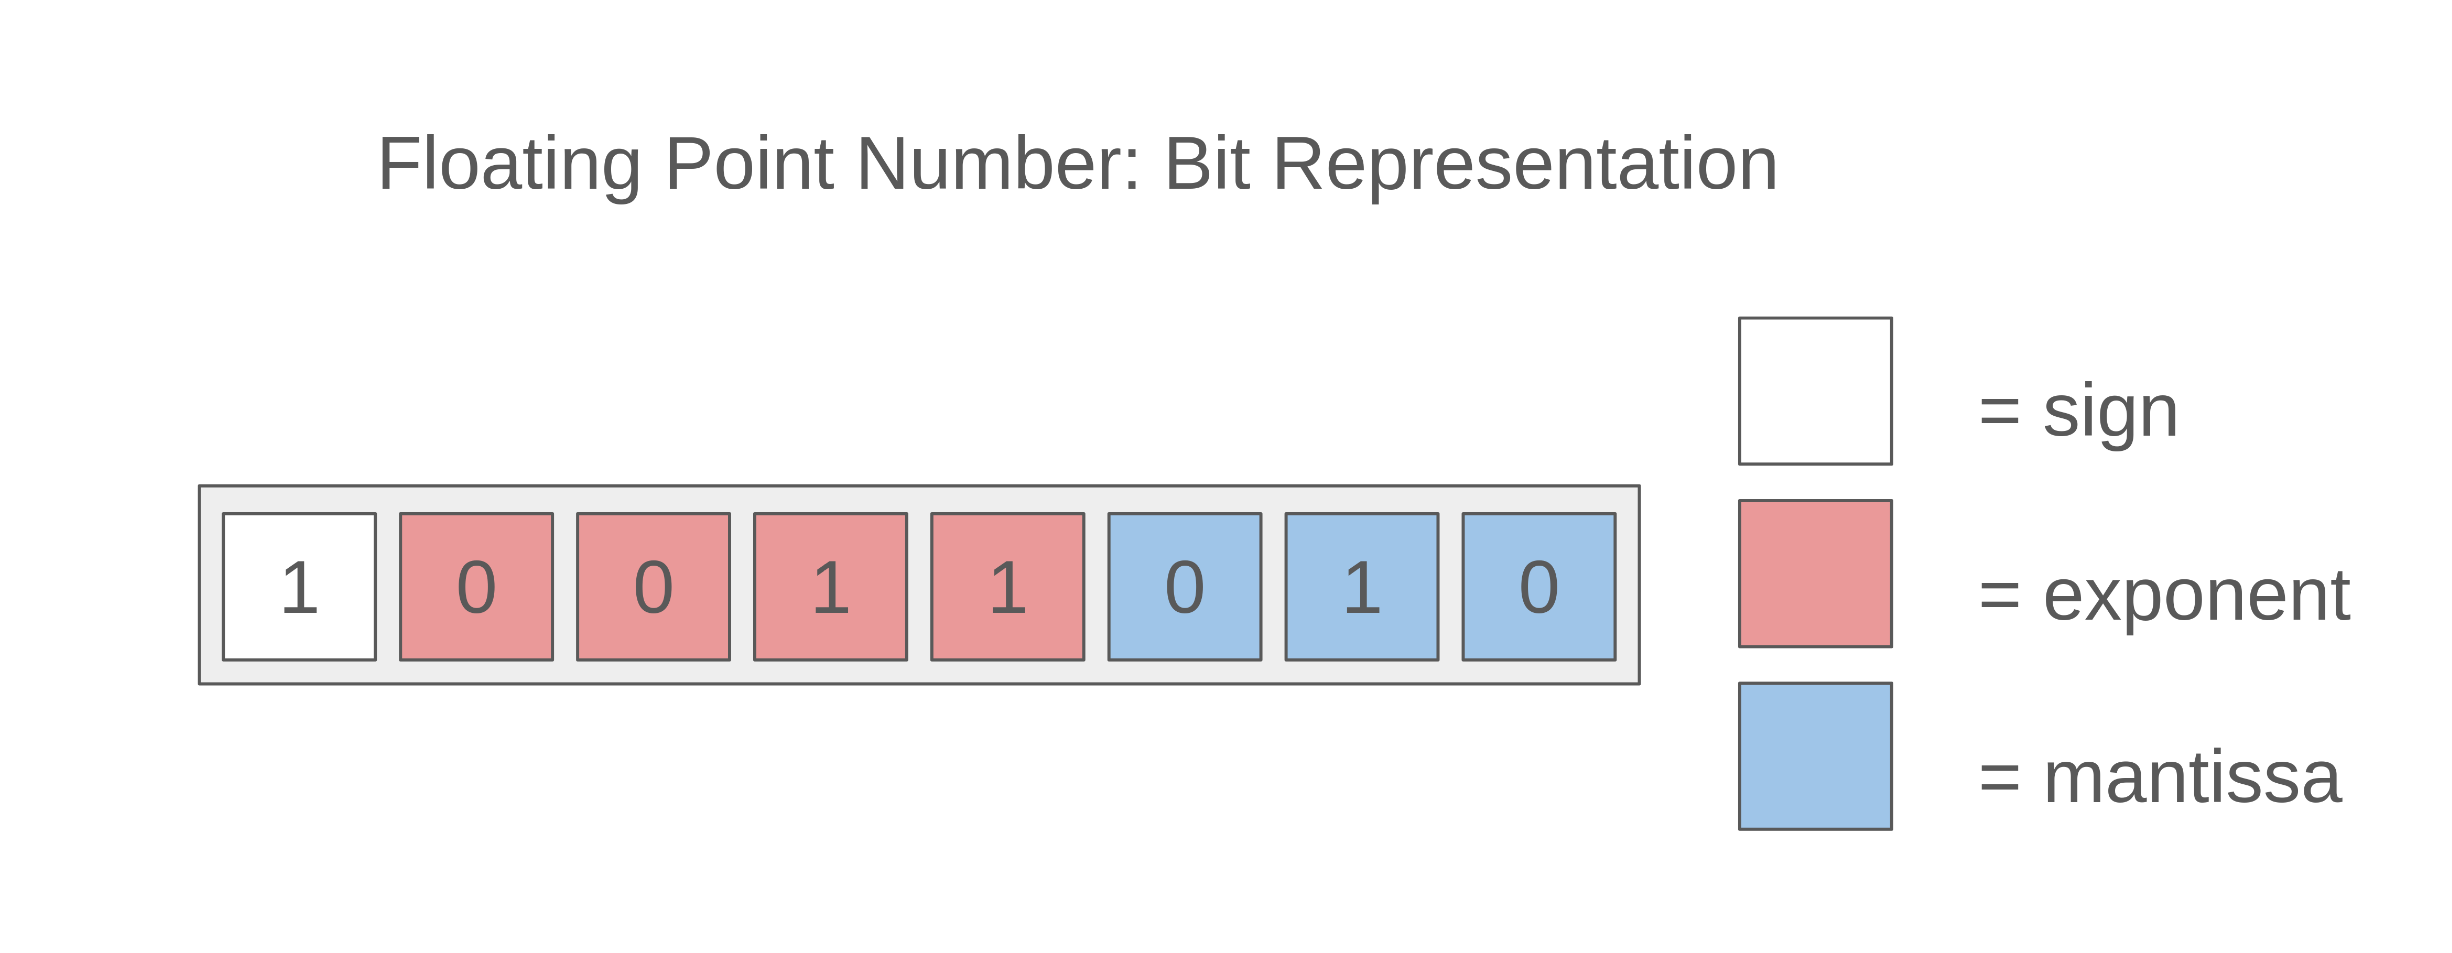
\includegraphics[width=0.5\linewidth]{Images/float_bit_representation.png}
    \caption{simplified floating point representation of a number, in this case the number 0.078125}
    \label{fig:float_bit_representation}
\end{figure}

Equation~\ref{eq:float} shows the equation that corresponds to the decimal value of a floating point number stored in this format. The IEEE 754-2008 Standard has predefined bit widths for the exponent and mantissa sections, this example disregards these sizes and operates with the sizes in figure~\ref{fig:float_bit_representation}

\begin{equation}\label{eq:float}
    (-1)^{bit_7} * 2^{(exponent) - 7} * mantissa \, value
\end{equation}

The sign bit decides whether the number is positive or not. The function of the bit is shown in equation~\ref{eq:float1}.

\begin{equation} \label{eq:float1}
    (-1)^{1} = -1
\end{equation}

The exponent part of the floating point number decides the exponent part of the equation. The IEEE standard defines the exponent part of the number using an implicit negative offset, such that if all exponent bits except the most significant bit (bit at index 6) in figure~\ref{fig:float_bit_representation}) are set to 1, the exponent is 0. For the arbitrary floating point format shown in figure~\ref{fig:float_bit_representation}, the offset becomes $2^4 - 1$, which is 7. This makes the exponent part of our arbitrary floating point number as shown in equation ~\ref{eq:float2}.
\begin{equation} \label{eq:float2}
    2^{4-7} = 2^{-3}
\end{equation}

The final part of the floating point number, the mantissa, also known as the fraction or the significand, is usually the largest part (with respect to the amount of bits in a binary representation it takes up) of a floating point number, but seeing as the floating point representation in figure~\ref{fig:float_bit_representation} is entirely of my invention I don't have to conform to those norms, though I will follow the same rules for calculating the value.
The value of the number is calculated as with an integer represented in binary, only starting at bit index 2 the bit value is $bit\,value*2^{-1}$, the value at bit index 1 is $bit\,value*2^{-2}$, and so on. Additionally, an implicit value of the integer 1 is added to the mantissa. This makes the value represented in figure~\ref{fig:float_bit_representation} shown in equation~\ref{eq:float3}:

\begin{equation}\label{eq:float3}
   1 + 0*2^{-1} + 1*2^{-2} + 0*2^{-3} = 1.25
\end{equation}

Plugging in the values found above into equation~\ref{eq:float} gives us $-1 * 2^{-3} * 1.25 = 0.078125$
The IEEE definitions have additional special cases for when all bits in the exponent are either 1 or 0 to deal with special situations, but this is not important for a basic understanding of how the bit representation works.

When reducing the size of the data you are operating on, for example replacing some of the double precision floating point values to single precision floating point values, the most significant change is that you are required to fetch and store less bits from memory, alleviating the storage bottle neck in processing~\citep{floatsmith_paper}.

\taffo{} also performs conversions from floating point number representations, but instead of switching between different bit widths of floating point numbers, \taffo{} transforms numbers to fixed point representation. Figure~\ref{fig:fixed_point_representation} shows an arbitrary number, and its complement (the same number multiplied by -1) in binary.

\begin{figure}
    \centering
    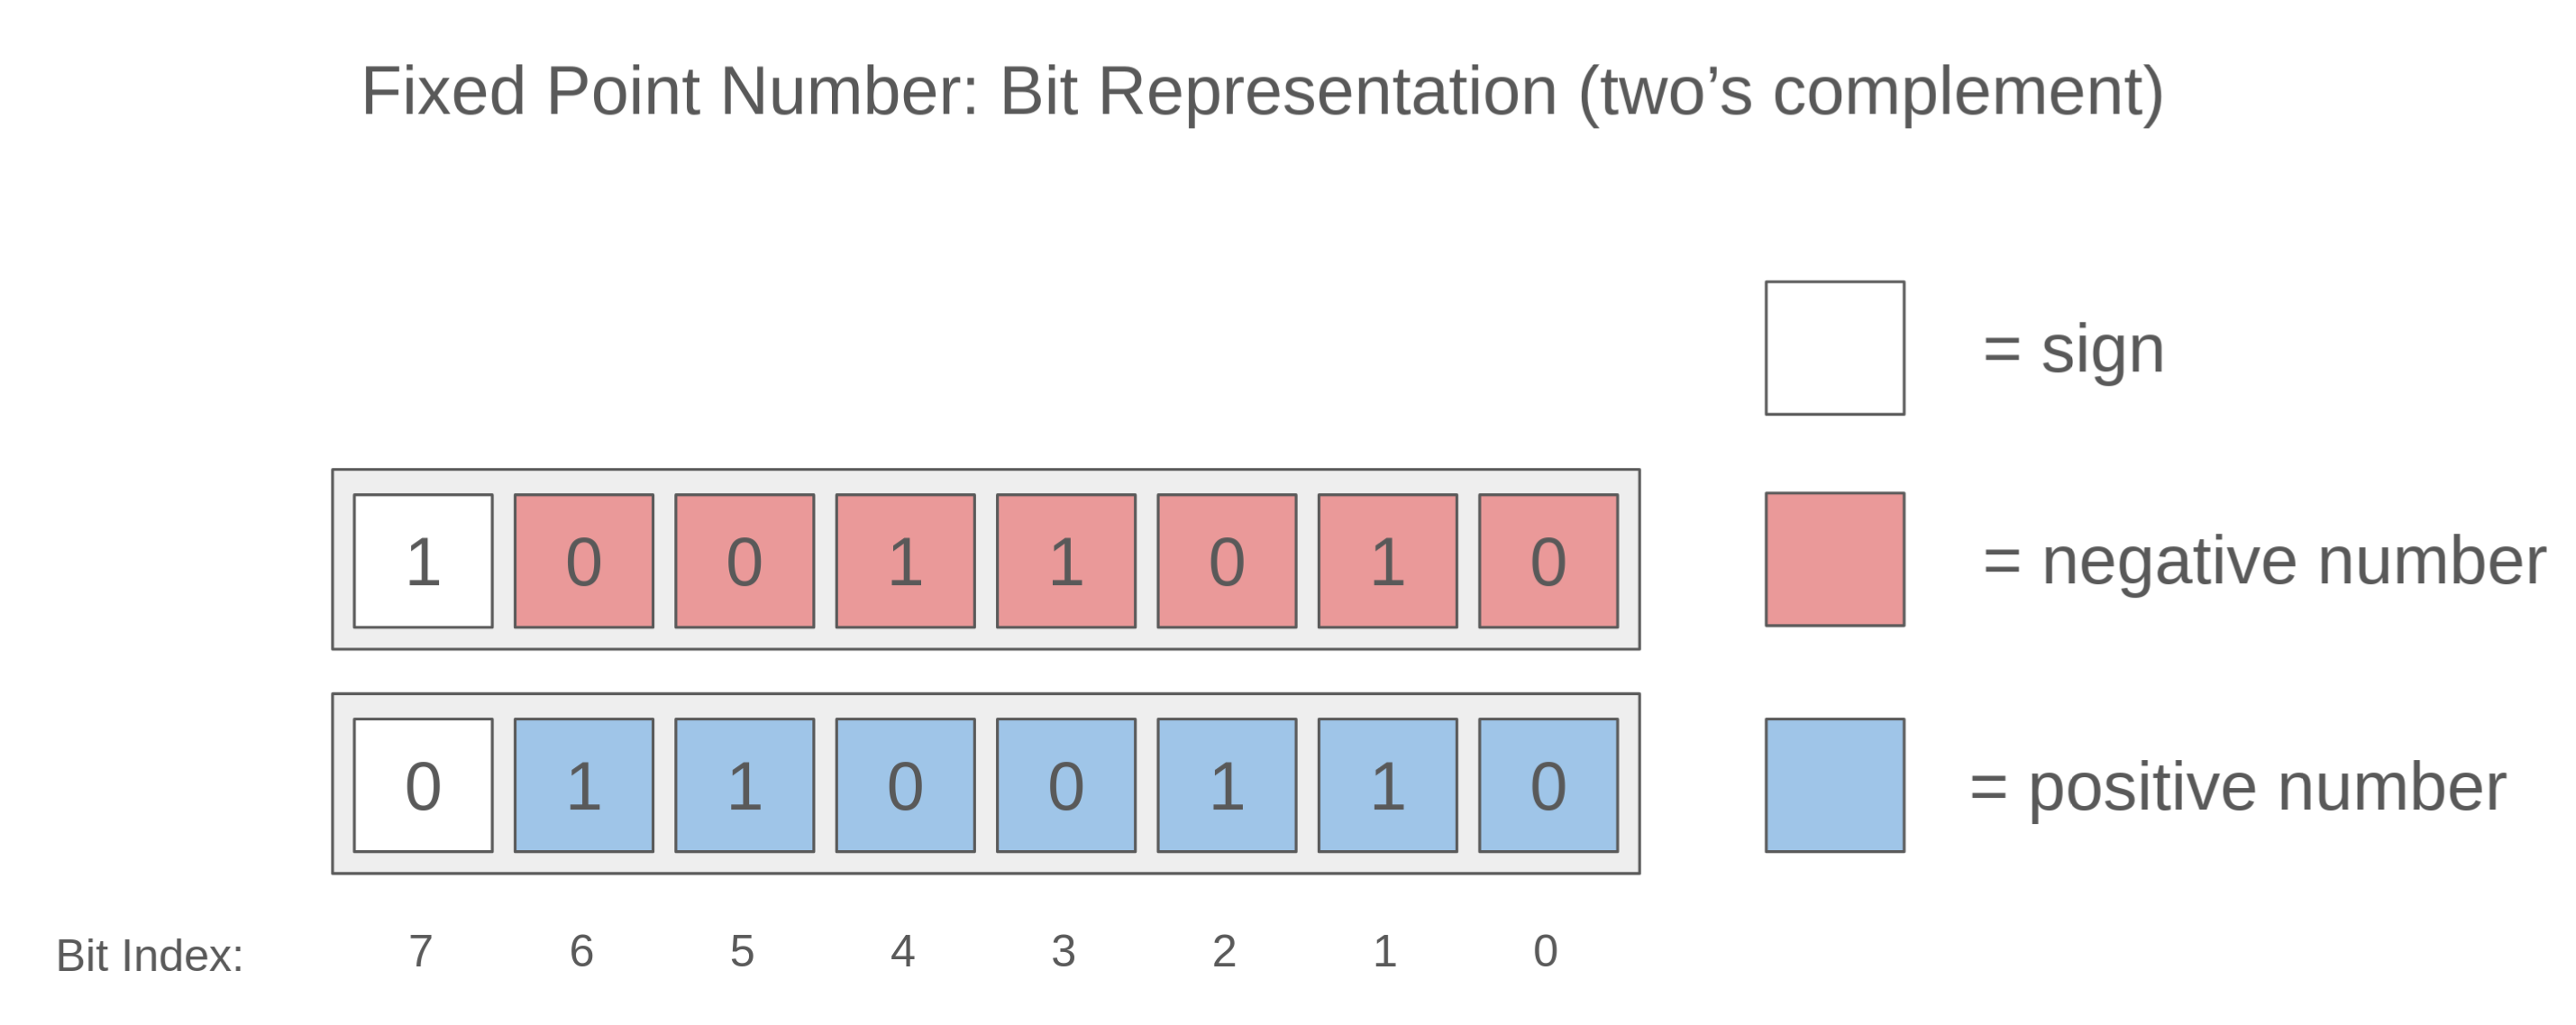
\includegraphics[width=0.5\linewidth]{Images/fixed_point_bit_representation.png}
    \caption{Fixed point representation of a number in binary. The figure shows one number and its complement, represented using the two's complement method.}
    \label{fig:fixed_point_representation}
\end{figure}

Fixed point numbers are represented by allocating a fixed amount of bits for the fractional part, and a fixed number of bits for the integer part. This is implicit and not visible in how a processor treats the numbers, which means that the processor can use the same hardware for operating on fixed point (fractional) numbers as regular integers, which is often speedier than performing operations on floating point numbers. It then becomes the programmers job to scale the number, often done by shifting the number to the left (which is equivalent to multiplying the number by $2^n$, $n$ being the amount of bits you are shifting the value.

Therefore, depending on the program, the numerical values for the bit representations in figure~\ref{fig:fixed_point_representation} could be 102 for the positive and -102 for the negative if we do not use a scaling factor, or if we decide that the three lower bits should be the fractional part of the number, to get our output number we must perform a right shift three places for the integer part of the number: 1100, which gives us the integer 12. The rightmost bits also have to be scaled by the same factor, i.e. $2^3$. To represent this as a decimal number requires us to divide by the scaling factor. 110 in binary is the same as 8 in integer representation. This gives us $6/8 = 0.75$, making the number represented 12.75.

Fixed point numbers can represent a smaller range of numbers with the same amount of bits as a floating point representation, and with lower precision. The flip side is that they are in general easier to perform computations on. 

\taffo{} therefore depends on users of the program to annotate a variable that is to be converted to a fixed point type with the range of values it can have, which is used to decide how many bits is required to represent the number accurately enough as a fixed point number. 

These two tools were selected as they were two of the few tools that had source code available on the internet without having to beg the authors in the paper for crumbs. 

There are other papers detailing different methods of approximate computing. Sadly, though they are described vividly in the papers, efforts to get a hold of these storied approximate computing tools proved fruitless. Though the tools described in the papers do not as far as I am concerned exist, the techniques exist, and can be applied manually.

\subsubsection{Approximate Computing through Loop Perforation}

Loop perforation, described in~\citet{li2018sculptor}, works by skipping iterations in loops that iteratively get closer to an accurate number. This would not necessarily work on just any loop, such as a loop reading in lines of data from a file, as this could cause data corruption.

\subsubsection{Approximate Computing through Memoization}

Memoization consists of mapping the inputs of expensive functions to their outputs, and avoiding to re-run the function for the same input, thereby saving energy. This is described more in depth by~\citet{mittal2016survey}.

\subsection{LLVM-IR}
LLVM-IR (LLVM Internal Representation) is an assembly-like programming language used as an intermediate representation within the LLVM suite of tools. LLVM is not an acronym, though in the early stages of the project it used to stand for Low Level Virtual Machine. These tools are mostly made for performing code transformations, and these transformations are made on LLVM-IR. The LLVM tools relevant to this thesis is the core optimizer for optimizing code, and clang for compiling C/C++~\citep{LLVM_homepage}.  %explain llvm 

\taffo{} is comprised of LLVM optimization passes. These optimization passes are performed on LLVM-IR, and clang is used to compile source code (with custom made annotations denoting the range of the variables) to LLVM-IR. %how taffo figures in this



\subsection{Reliability through Fault Tolerance}\label{section:Reliability_thorugh_fault_tolerance}
Reliability is a concept that concerns itself with whether a system provides correct service or not. A system in this context could be a software component such as a software library, or an entire computer system together with software such as an ATM machine. Correct and incorrect service is not necessarily a rigid concept for all types of systems. In the case of an ATM machine, correct service requires cash withdrawals to match the amount withdrawn from an account exactly for the service to be defined as correct, while a computer vision face detection library that detects a face in 90 out of 100 images may still be considered to provide correct service.

\citet{avizienis2004basic} provides this definition of reliability, as well as dividing reliability into multiple related concepts. Of these, the most relevant to this thesis is the definitions of fault tolerance, service failure, errors, and faults.  

Fault tolerance is a prerequisite to reliability. Fault tolerance is defined as the continued delivery of correct service in spite of faults present in the system. A fault is an artifact that may result in an error, and an error is an internal state of the system, or a part of the system, that deviates from correct service. An error does not necessarily end up affecting the external state (the output of the system, or system delivery), but the moment that an error does affect the external state to an incorrect state, this constitutes a service failure.

\citet{avizienis2004basic} divides faults into two categories: developmental faults, or operational faults. Faults are divided into one of the two depending on when they occur: developmental faults occur during the development of the system, and operational faults occur when the system is providing service. A software bug would be a developmental fault, and a bit flip caused by ionizing radiation would constitute an operational fault.

\subsubsection{Verifying Fault Tolerance}\label{section:Verifying_fault_tolerance}

Different applications have different fault tolerance requirements; a satellite in orbit of the earth would necessarily have much higher requirements with respect to operational fault tolerance than a run-of-the-mill home computer. Developmental fault tolerance in software governing an industrial complex will also be stricter than the software governing a smart home system. 

Given these requirements, one way of verifying or quantifying the fault tolerance of a system is through fault injection. There are frameworks for injecting both operational and developmental faults allowing users to gauge fault tolerance in a way that would be difficult without: Given a lack of the resources required to perform hardware fault injection as~\citet{arlat1993fault} describe, software alternatives like Xception~\citep{carreira1998xception} that allows the user to emulate hardware bit flips in a program, or the Gem5-approxilyzer described in~\citet{venkatagiri2019gem5} that allows users to simulate how single bit flips propagate instruction by instruction through a processor can provide accurate alternatives.

Developmental fault injection can also be performed, with~\citet{natella2012fault} describing an approach using available statistics for a category of software to infer potential fault locations that statistically would not be caught in testing. Injecting faults that are caught by tests to evaluate tests is a strategy commonly known as mutation testing, the goal of which is to create code "mutants" (versions of your code that contain an injected error), and then "killing" the mutants with the test suite, i.e.,  the test suite catches unexpected behavior through tests failing.

\cleardoublepage


\chapter{Method}
\section{Method}

The goal of this thesis was to gauge the fault tolerance of approximate computing tools using fault injection. The faults in question were injected in software for practical reasons as hardware fault injection requires significantly more effort, and in LLVM bytecode in an effort to make the results applicable regardless of programming language.

The tools that were tested were floatsmith and \taffo{}.

Prerequisite to testing the tools is installing the tools. \taffo{} depends on LLVM 14 or 15 to run, and is at the time of writing not compatible with newer versions of LLVM (the most recent version is 20). To install LLVM 15 you can build it from the source code following the instructions found at the llvm website, \href{llvm.org}{llvm.org}. On certain GNU/linux distributions you may also install llvm through your package manager (if supported by the LLVM organization), but you may need to add the LLVM repository  to your package manager of choice for this to work. 

Building \taffo{} was only successful when using pre-built binaries. 
The other tool that was used was floatsmith. This can be installed the easiest using their provided docker image, and mounting the project you want to perform experiments on.

\subsection{Bitwise fault injection}
Bitwise fault injection was done thorugh manually performing an XOR operation in LLVM IR on the values to be subjected to faults. Table~\ref{table:xor_truth_table} shows the truth table for two bit inputs through an XOR-gate. The output is 1 if and only if either input A or input B is 1 while the other is 0. If using input B as a bit mask of which bits to flip, we can see in the table that the output becomes the opposite of input A for all cases of input B being 1, and when input B is 0 all outputs are the same as input A. Such an operation on two 8-bit numbers is shown in figure~\ref{fig:xor_operation}. The output of the XOR operation shows that the output is the same as the input, except for the bit that is marked with red, which has been flipped.

\begin{table}[htb]
    \centering
\caption{Truth table for XOR function}
    \label{table:xor_truth_table}
\begin{tabular}{c|c|c}\label{table:xor_truth_table}
     input A& input B& XOR output \\
     0&0&0\\
     1&0&1\\
     0&1&1\\
     1&1&0
\end{tabular}
    
\end{table}



\begin{figure}[h!]
    \centering
    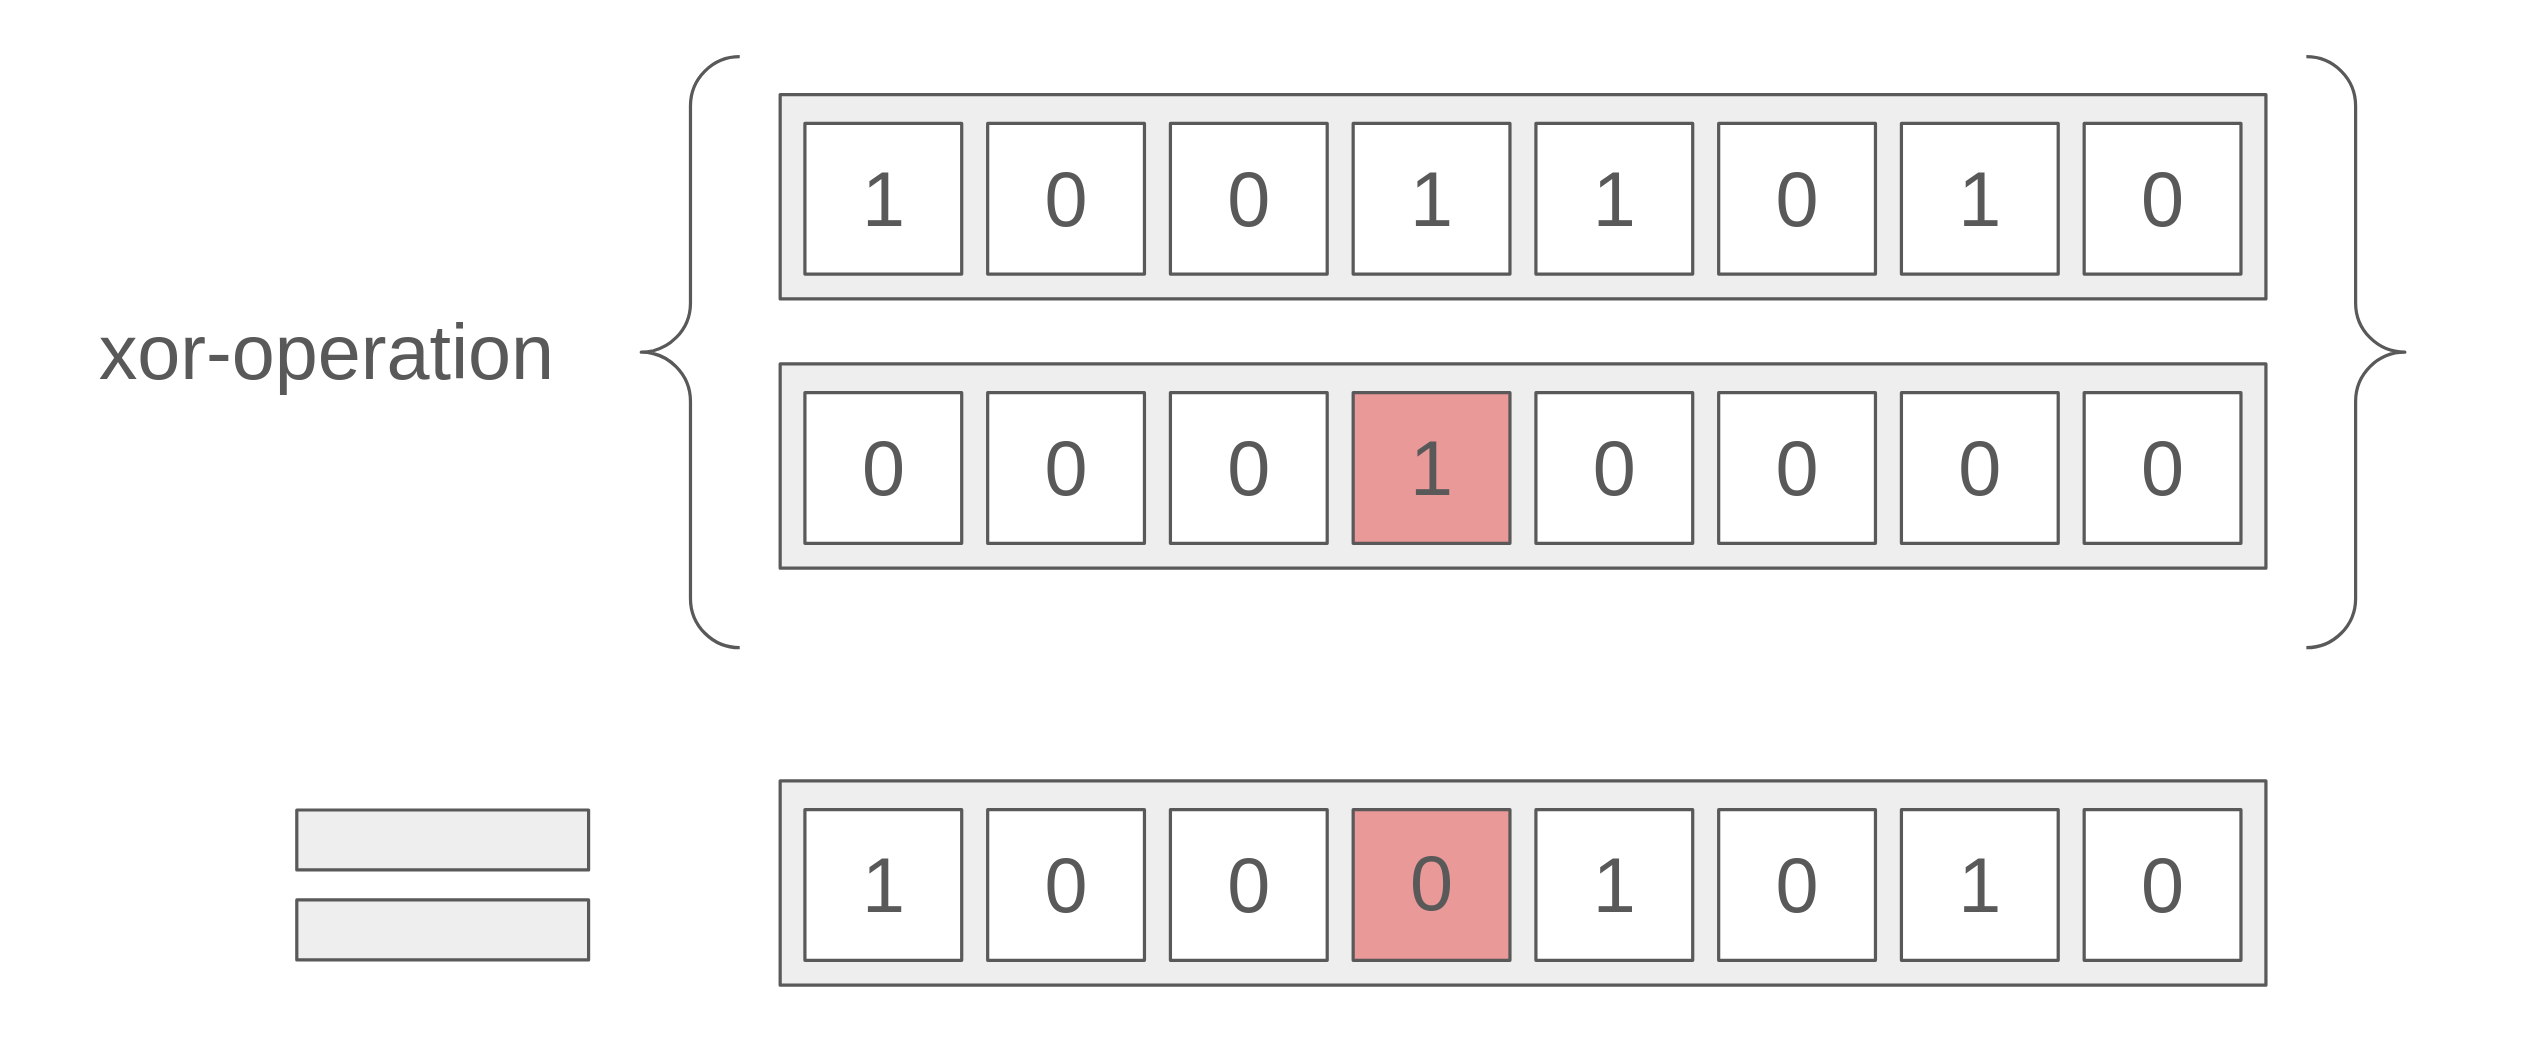
\includegraphics[width=0.5\linewidth]{Images/xor_operation.png}
    \caption{An example XOR operation between two numbers.}
    \label{fig:xor_operation}
\end{figure}

This was applied directly in LLVM bytecode using LLVM bytecode commands to perform a bit flip on a data variable in the program. Code listing~\ref{listing:llvm_ir_fixed} shows how the bit flip was implemented for the fixed point implementation, and listing~\ref{listing:llvm_ir_float} shows the bitflip for the floating point implementation.



The result of a division is selected as the value to perform fault injection on as there are only two division operations in the benchmark source code, one in the data generation part of the code, and one in the main computational kernel. These two division operations can be distinguished from each other through the fact that the division in the main computational kernel divides a variable by the constant value 9. This constant value is preserved directly in LLVM bytecode, which makes it trivial to find the division operation in the data preparation kernel.\footnote{The fixed point implementation actually contains three division operations, of which one is a floating point division. The origin of this floating point division operation is unclear, but it can be safely disregarded for the purposes of this fault injection campaign.}
Two temporary variables, \%temp1 and \%temp2, are introduced, where \%temp1 is a 64 bit integer with value 1 shifted left however many bits necessary to inject a bit in the desired location. Listing~\ref{listing:llvm_ir_fixed} injects a bit in bit index number 4, making the last 8 bits of \%temp1 look like the mask number (with the bit highlighted in red) shown in figure~\ref{fig:xor_operation}.
The variable \%temp2 stores the result of the XOR operation between the result of the division in \%18 and the bit mask from \%temp1, and is then placed where \%18 ordinarily would be in the variable \%s10\_22fixp4.

\begin{lstlisting}[caption=fixed point bit flip in LLVM bytecode, label=listing:llvm_ir_fixed]
  %17 = sext i32 %0 to i64, !taffo.info !45
  %18 = sdiv i64 %16, %17, !taffo.info !109
  %temp1 = shl i64 1, 4
  %temp2 = xor i64 %temp1, %18
  %s10_22fixp4 = trunc i64 %temp2 to i32, !taffo.info !110
\end{lstlisting} 

\begin{lstlisting}[caption=floating point bit flip in LLVM bytecode, label=listing:llvm_ir_float]
  %temp1 = fdiv double %24, %26
  %temp2 = shl i64 1, 4
  %temp3 = bitcast double %temp1 to i64
  %temp4 = xor i64 %temp2, %temp3
  %27 = bitcast i64 %temp4 to double
\end{lstlisting}

Flipping a bit in the floating point implementation requires first performing a bitcast operation on the floating point number to be fault injected, \%temp1 in listing~\ref{listing:llvm_ir_float}. This means simply marking the bits in the memory location of \%temp1 as an integer, without actually changing any of the bits. This has to be done because the number 1 stored as a fixed point number is all zeros except the least significant bit which is 1, and a floating point binary representation contains several bits set to 1 in the exponent part of the number due to the exponent offset, see~\ref{section:approximate_computing_through_reducing_bits}. After the fault injection is performed, the fault injected variable then needs to be bitcast back to a floating point number.

The first fault injection campaign consisted of single bit fault injections. This consisted of taking a sample benchmark from the \taffo{} repository, compiling it to an intermediate format, in this case the LLVM IR, then flipping single bits one location at a time, and building it to a fault injected executable. For \taffo{}, which converts floating point values to lower precision fixed point values, this requires creating a fault injected version for both the fixed and floating point intermediate format.

For each pair of fault injected executables, the outputs are compared between each other and the original floating point implementation.

To streamline injections a helper script was created based on the existing scripts in the \taffo{} repository. This allows a user to compile the selected benchmark from a list of benchmarks to LLVM IR, inject faults in a user-selected location in the code, then change the bit location of this fault, and compile many different versions of the same benchmark with different faults injected in the same location. The script then runs all the benchmarks and collects output. Finally a python script that reads these outputs collects and compares them in a human readable format. To use the script, the user needs to manually set the range of bits that are being flipped in the run script. 

The comparison script written in python was written in a separate repository with tests, and iteratively copied over to the \taffo{} repository as development progressed. It was written to compare one single benchmark at a time, and this is documented in the repository. To enable automatically making an overview of fault injection on multiple different benchmarks at the same time, changing the code is required. see the appendix for the link to the repository.



% her skrive om mutation-isj testing i taffo


\cleardoublepage


\chapter{Results}

The results of the thesis work consist of a fault injection campaign on a benchmark included in the \taffo{} repository and code additions. These additions reside in a clone of the \taffo{} repository hosted on \href{https://github.com/larsj-blip/TAFFO}{https://github.com/larsj-blip/TAFFO}. The results include the experiences gathered from using \taffo{} and floatsmith to compile a test benchmark.


\section{Taffo}
The most significant results of the fault injection for a single benchmark can be found in table~\ref{table:injection_results}. The complete output can be found in appendix~\ref{appendix:complete_injection_results}. Outputs from the polybench benchmarks are stored in text files as string sequences of decimals separated by spaces. Taking the outputs from the floating point without injected faults as the control, the element by element difference between the control and the fault injected program versions is added up, and divided by the amount of data points to get the average difference for all output values. Table~\ref{table:injection_results} shows the average difference per data point between the output files of the fault injected versions and the unmodified floating point version.   
The first column shows the filename where the output from the executable is stored. The filename is built from the benchmark name, which in this case is seidel-2d. The next part of file name contains the location of the injected bit in the variable, with "bit\_no\_0" representing a bit flip in the least significant bit of the variable (at index 0). The final part of the filename specifies whether the file output stems from a floating point implementation or a fixed point implementation.
The first fixed point implementation of the benchmark without any faults injected is an exception, this is the entry with filename seidel-2d.txt.

The second column shows the result of the above mentioned comparison between the unmodified floating point implementation of the benchmark, seidel-2d, and the implementation specified in the leftmost column. 

%  DETTE VAR REPETISJON The value is calculated by taking the absolute value of the difference of each value at index [x] for all values of x, and dividing the accumulated difference by the amount of values. This gives the average difference per data point between the two outputs.

The values in column three are redundant and are present only for consistency with the actual output of the comparison script. For a given fault injection location, column three shows the comparison results for the alternative implementation of the program. For example, the value in column three for the entry seidel-2d\_bit\_no\_0.fixed.txt is the same as the value in column two in the entry at seidel-2d\_bit\_no\_0.float.txt. This was done because this was quicker than implementing sorting for the print function in the comparison script. The outputs in listing~\ref{table:injection_results} and in appendix~\ref{appendix:complete_injection_results} are ordered manually.


%\begin{longtable}{lll}
\begin{table}
\caption{The table shows the output of the simple python script that collects the absolute differences between the original floating point implementation and the fault injected versions of the benchmark.}
\label{table:injection_results}
\begin{tabular}{lll}
   

{\bf Filename} & {\bf Average Difference} & {\bf Alternative } \\
       ~      & {\bf From Control }      & {\bf Implementation Results}\\
 \hline
    seidel-2d.float.txt & 0.0   & 0.00010252590179347587 \\
    seidel-2d.txt & 0.00010252590179347587 & 0.0 \\
    seidel-2d\_bit\_no\_0.fixed.txt & 0.00010252738737963263 & 4.526846432428844e-15  \\
    seidel-2d\_bit\_no\_0.float.txt &  4.526846432428844e-15 & 0.00010252738737963263 \\
    seidel-2d\_bit\_no\_1.fixed.txt & 0.00010252973353766834 & 7.836499591601375e-15 \\
    seidel-2d\_bit\_no\_1.float.txt & 7.836499591601375e-15 & 0.00010252973353766834 \\
    seidel-2d\_bit\_no\_2.fixed.txt & 0.00010242978918456464 & 1.0070183402433041e-14 \\
    seidel-2d\_bit\_no\_2.float.txt & 1.0070183402433041e-14 & 0.00010242978918456464 \\
    seidel-2d\_bit\_no\_3.fixed.txt & 0.00010269591987037501 & 1.7122632695390493e-14 \\
    seidel-2d\_bit\_no\_3.float.txt & 1.7122632695390493e-14 & 0.00010269591987037501 \\
    seidel-2d\_bit\_no\_30.fixed.txt & 240.38767306192983 & 8.453350257722744e-07 \\
    seidel-2d\_bit\_no\_30.float.txt & 8.453350257722744e-07 & 240.38767306192983 \\
    seidel-2d\_bit\_no\_31.fixed.txt & 432.92573090152945 & 2.020661384195993e-06 \\
    seidel-2d\_bit\_no\_31.float.txt & 2.020661384195993e-06 & 432.92573090152945 \\
    seidel-2d\_bit\_no\_32.fixed.txt & 0.00010252590179347587 & 6.188653891382238e-06 \\
    seidel-2d\_bit\_no\_32.float.txt & 6.188653891382238e-06 & 0.00010252590179347587 \\
    seidel-2d\_bit\_no\_60.fixed.txt & 0.00010252590179347587 & 1.1633619119162309e+79 \\
    seidel-2d\_bit\_no\_60.float.txt & 1.1633619119162309e+79 & 0.00010252590179347587 \\
    seidel-2d\_bit\_no\_61.fixed.txt & 0.00010252590179347587 & 1.3470810631989899e+156 \\
    seidel-2d\_bit\_no\_61.float.txt & 1.3470810631989899e+156 & 0.00010252590179347587 \\
    seidel-2d\_bit\_no\_62.fixed.txt & 0.00010252590179347587 & nan \\
    seidel-2d\_bit\_no\_62.float.txt & nan   & 0.00010252590179347587 \\
    seidel-2d\_bit\_no\_63.fixed.txt & 0.00010252590179347587 & 201.00625000002313 \\
    seidel-2d\_bit\_no\_63.float.txt & 201.00625000002313 & 0.00010252590179347587 \\
    \end{tabular}%
%  \label{tab:addlabel}%
%\end{longtable}%
\end{table}


The control, seidel-2d.float.txt, is identical to itself, so the difference is 0.0. Initially the fixed point difference is many orders of magnitude larger than the floating point difference, for the result from injected bit at index 0, the average difference between fixed point and control is larger by an order of magnitude of 11 compared to the difference between the floating point implementation. 

After bit number 54, the floating point average difference grows substantially from the previous bit injection, from 140.41412113413136 to 25619.825047812476, which is a factor of over 182. At this point, assuming that the floating point implementation follows the IEEE 754 standard, the bits flipped are in the exponent part of the floating point representation, which makes sense with the increase in size. The result for injected bit at index 62 is undefined for the floating point implementation, due to many NaN (not a number) outputs. There is no observed change in the fixed point output data compared to the original fixed point computation from injected bit at index 32 until injected bit at index 63.


When building \taffo{}  succeeded, the next goal was to use the existing framework provided in the benchmarks modified for use with \taffo{} to perform fault injection. There is an existing validate.py python script used to compare the standard floating point implementations of the polybench benchmarks and \taffo{}-produced fixed point implementations, and this was used to gain a basic understanding of how the outputs of the benchmarks were used to evaluate the performance and error of the \taffo{} code transformations. Line by line the code was refactored to be more verbose, and to more clearly represent the actions happening in the script.
Listing~\ref{lst:validate_original} shows one of the functions in the original script, and listing~\ref{lst:validate_new} shows the refactored version. The refactored version is functionally equivalent to the original and provides the same output, save for modified dictionary keys in the output. This is because the script uses the dictionary keys as headings. 




\begin{lstlisting}[language=python,label=lst:validate_new,caption=Validate new]
def compute_difference(fixed_point_data, floating_point_data):
    successful_iterations = 0
    total_difference_floating_and_fixed_point_values = Decimal(0)
    total_floating_point_value = Decimal(0)
    fixed_point_invalid_result_count = 0
    floating_point_invalid_result_count = 0
    error_threshold = Decimal('0.01')

    for single_value_fixed_point, single_value_floating_point in zip(fixed_point_data, floating_point_data):
        fixed_point_value, floating_point_value = Decimal(single_value_fixed_point), Decimal(
            single_value_floating_point)

        if not fixed_point_value.is_finite():
            fixed_point_invalid_result_count += 1
        elif not floating_point_value.is_finite():
            floating_point_invalid_result_count += 1
            fixed_point_invalid_result_count += 1
        elif ((floating_point_value + fixed_point_value).copy_abs() - (
                floating_point_value.copy_abs() + fixed_point_value.copy_abs())) > error_threshold:
            fixed_point_invalid_result_count += 1
        else:
            successful_iterations += 1
            total_difference_floating_and_fixed_point_values += (
                        floating_point_value - fixed_point_value).copy_abs()
            total_floating_point_value += floating_point_value

    average_error_percentage = (
                total_difference_floating_and_fixed_point_values / total_floating_point_value * 100) \
        if total_floating_point_value != 0 and successful_iterations > 0 else -1
    average_absolute_error = (
                total_difference_floating_and_fixed_point_values / successful_iterations) \
        if successful_iterations > 0 else -1

    return {
        'fixed_point_invalid_result_count': 
            fixed_point_invalid_result_count if successful_iterations > 0 else "no successful iterations",
        'floating_point_invalid_result_count': 
            floating_point_invalid_result_count if successful_iterations > 0 else "no successful iterations",
        'avg_percentage_error': 
            str(
            average_error_percentage) + " %" if average_error_percentage != -1 else "no successful iterations",
        'avg_absolute_error': average_absolute_error if average_absolute_error != -1 else "no successful iterations"}

\end{lstlisting} 


\begin{lstlisting}[label=lst:validate_original,caption=Validate original,language=python]
def ComputeDifference(fix_data, flt_data):
  n = 0
  accerr = Decimal(0)
  accval = Decimal(0)
  fix_nofl = 0
  flo_nofl = 0

  thres_ofl_cp = Decimal('0.01')

  for svfix, svflo in zip(fix_data, flt_data):
    vfix, vflo = Decimal(svfix), Decimal(svflo)

    if not vfix.is_finite():
      fix_nofl += 1
    elif not vflo.is_finite():
      flo_nofl += 1
      fix_nofl += 1
    elif ((vflo + vfix).copy_abs() - (vflo.copy_abs() + vfix.copy_abs())) > thres_ofl_cp:
      fix_nofl += 1
    else:
      n += 1
      accerr += (vflo - vfix).copy_abs()
      accval += vflo
      
  e_perc = (accerr / accval * 100) if accval != 0 and n > 0 else -1
  e_abs = (accerr / n) if n > 0 else -1
      
  return {'fix_nofl': fix_nofl, \
          'flo_nofl': flo_nofl, \
          'e_perc': e_perc,
          'e_abs': e_abs}
\end{lstlisting}




The comparison python script that was used to create the results in listing~\ref{lst:injection_results} was written in a separate github repository, and transplanted over to the \taffo{} repository whenever it was updated. This was done out of percieved convenience, but the directory with the script and the tests might just as well have been located in the taffo repository. In hindsight, this is probably also easier.

The comparison script was written with tests documenting the behavior, and comments pointing out missing tests and undocumented behavior. Especially the tests are vital for external programmers to understand the intent behind the code, and more tests would have made it easier to understand the existing behavior in the \taffo{} repository. 

The edited scripts for compilatoins and running the benchmarks were heavily influenced by the existing compile.sh and run.sh scripts located in the tests/polybench-cpu directory, but edited for the purposes of this thesis. The new script for running the benchmarks provided functionality to run multiple files of the same benchmark with bitwise faults injected at different locations, and the new compile script likewise allows the user to easily compile multiple versions of the same script with bitwise faults at different locations. Instructions on the use of these scripts to repeat/extend the experiment is contained within the scripts themselves.


\section{Floatsmith}

Floatsmith was selected as an option for fault injection campaigns along with \taffo{} because of source code being available, and the program being installable through a docker image. Initial studies of floatsmith were promising, as transforming the code included in the demos was easy. 
However, when attempting to apply floatsmith to the benchmark code located in \taffo{} the result was an error, and no hints as to what may have been the problem. In the paper detailing floatsmith, the authors state that the tool has not been tested on larger codebases, and this may be a part of the problem. The demo scripts that comes with the floatsmith installation are single file programs, while the polybench benchmarks that come with \taffo{} are all multi-file programs. This, together with outdated/lacking documentation (for instance, at the moment there are dead links in the repository README), lead to no numerical results, but this in itself is a result.



\cleardoublepage


\chapter{Discussion}
\section{Discussion}

\subsection{Fault Injection Method}

The fault injection campaign was intended to begin at a higher abstraction level than LLVM bytecode through injecting errors in the benchmarks' source C code. These initial efforts consisted of performing an equivalent of mutation testing in the selected benchmark. This was largely misguided, as mutation testing does not make sense when it is not used to validate a test suite. 

Performing mutation testing in the tests that assert the behavior of taffo would allow discussing the developmental fault tolerance of \taffo{}, but this was hindered by the authors lack of experience with \taffo{} development and the test cases and assertions not being verbose and descriptive enough for an outsider to easily understand what the code was testing. Taking the test in listing~\ref{listing:taffo_unit_test} as an example, one can see that there is a variable annotated for use with taffo, and other variables that are not annotated. A value is returned, but there are no hints as to what the expected behavior given an input is. The function names don't help with this either, nor does the filename, which is test1.c. This makes performing mutation testing a lot more difficult. Mutation testing is used to verify that the tests actually test the behavior they describe, but when the behavior that is being tested is not described, it is all the more difficult to create mutants that target the test in question.

The README file in the simple-test-cases directory in taffo directs a potential tester to a shell script that builds and runs the test, and in the makefile the directory is marked as tests, running all the tests in the simple-test-cases directory when building taffo.

\begin{lstlisting}
    ///TAFFO_TEST_ARGS -Xvra -propagate-all


float global;

float test(float param, int notafloat)
{
  int notafloat2;
  float local __attribute((annotate("scalar(range(0, 5.0))")));
  
  local = 2.0;
  local *= param;
  local += notafloat;
  notafloat2 = local;
  return notafloat2;
}

int test2(int a)
{
  return a + 2.0;
}

\end{lstlisting}

Instead of performing mutation testing on uncertain ground, the initial fault injection was performed directly in LLVM bytecode through the above mentioned single bit flip experiment.

\subsection{Fault Injection Bit Flip Campaign}

This comparison is based on injecting faults within the data that is being operated on, not on opcodes or memory locations. This is to verify the change in behavior that changing the variable type incurs.

The fault injection location was selected based on operations that are only done a few of in the program, such as division, to be able to inject a fault in an equivalent location for all the different versions of the program. The comparison does not hold for anything other than an injection of faults in the data. Furthermore the fault injection has only been performed on one benchmark with a limited number of operations, therefore the results may be different in another benchmark stressing another part of the processor. This is partly due to the fact that fixed point and floating point representations require different CPU instructions for mathematical operations. This leads to different code that uses different parts of the processor. 


The results of the fault injection campaign completed for the seidel-2d benchmark from the polybench cpu benchmark suite adapted for \taffo{} is not representative for programs compiled with \taffo{} as a whole. The changes that are made to the low-level code vary from project to project depending on the domain, and depends on what the user of the program specifies to be the range of values. 

The results from the fault injection were mostly expected: The deviations from the original answer for the floating point errors started low, then skyrocketed exponentially towards the most significant bits.




% explanation of floating point implementation
% explanation of fixed point implementatoin
% diagrams


In the output file of the original floating point implementation without any additional faults injected, there are 19 significant digits, 16 of which is behind the decimal point. Depending on what the output is used for, an error above 1.0 could be considered to be quite a large error, or it could be insignificant. Figure~\ref{fig:graph_fixed_vs_float_error} shows a graph of the change in error when injecting an error in increasingly more significant bits in a variable. The graph cut-off is set at 1.0, this is to get a better resolution in the lower end of the fault spectrum. The deviation is the accumulated average absolute difference for each data point compared to the original floating point implementation of the program without additional faults injected. The x axis describes which bit is flipped, bit number 0 being the least significant bit.

\begin{figure}[h!]
    \centering
    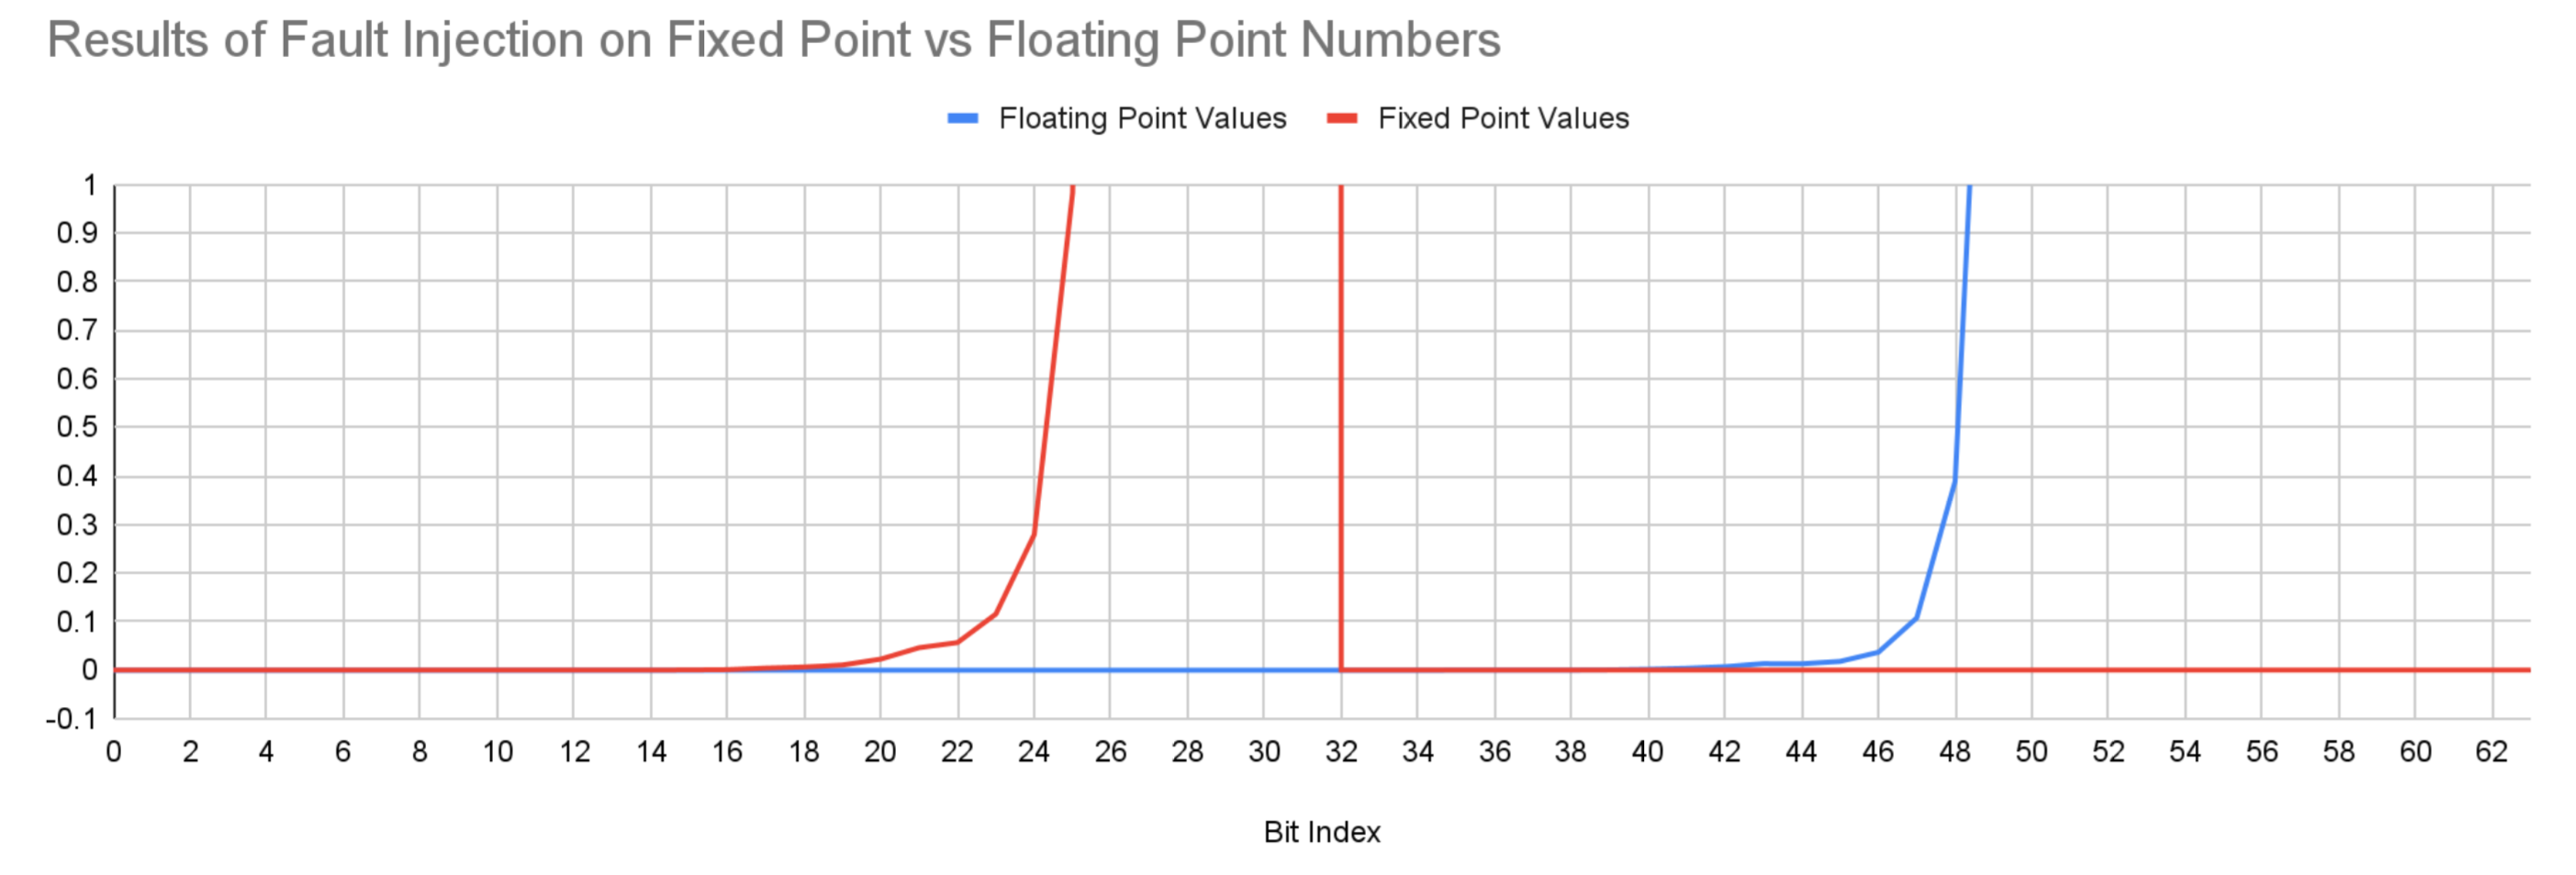
\includegraphics[width=0.5\linewidth]{Images/graph_float_vs_fixed_fault_injection_results.png}
    \caption{The graph shows how the difference from the original floating point version of the program increases the closer to the most significant bit the fault is injected. }
    \label{fig:graph_fixed_vs_float_error}
\end{figure}


The graph y axis starts at negative values even though this is not possible (the y axis is average absolute difference, therefore values will only be positive).This is to more clearly show the line for the floating and fixed point data when the error is small toward the least significant bits.

The graph shows that both the floating point values and the fixed point values seem to differ very little from the original non-fault-injected outputs. The difference in the fixed point implementation rises quickly as the injected bit approaches the the most significant bit, until suddenly dropping after injection in the bit at index 32. This can be explained by looking at the LLVM bytecode that is used to inject the faults, see listing~\ref{listing:llvm_ir_fixed}. Here you can see that while the result of the division is 64 bits, from dividing two 64 bit variables, one of the operands is originally a 32 bit integer that is extended to a 64 bit number. In the final line in the listing, the result of the division and bit flip is then truncated back to a 32 bit integer, thereby discarding the injected bit if it is injected over the bit at index 31, explaining the drop in error after bit 31.

\begin{figure}[h!]
    \centering
    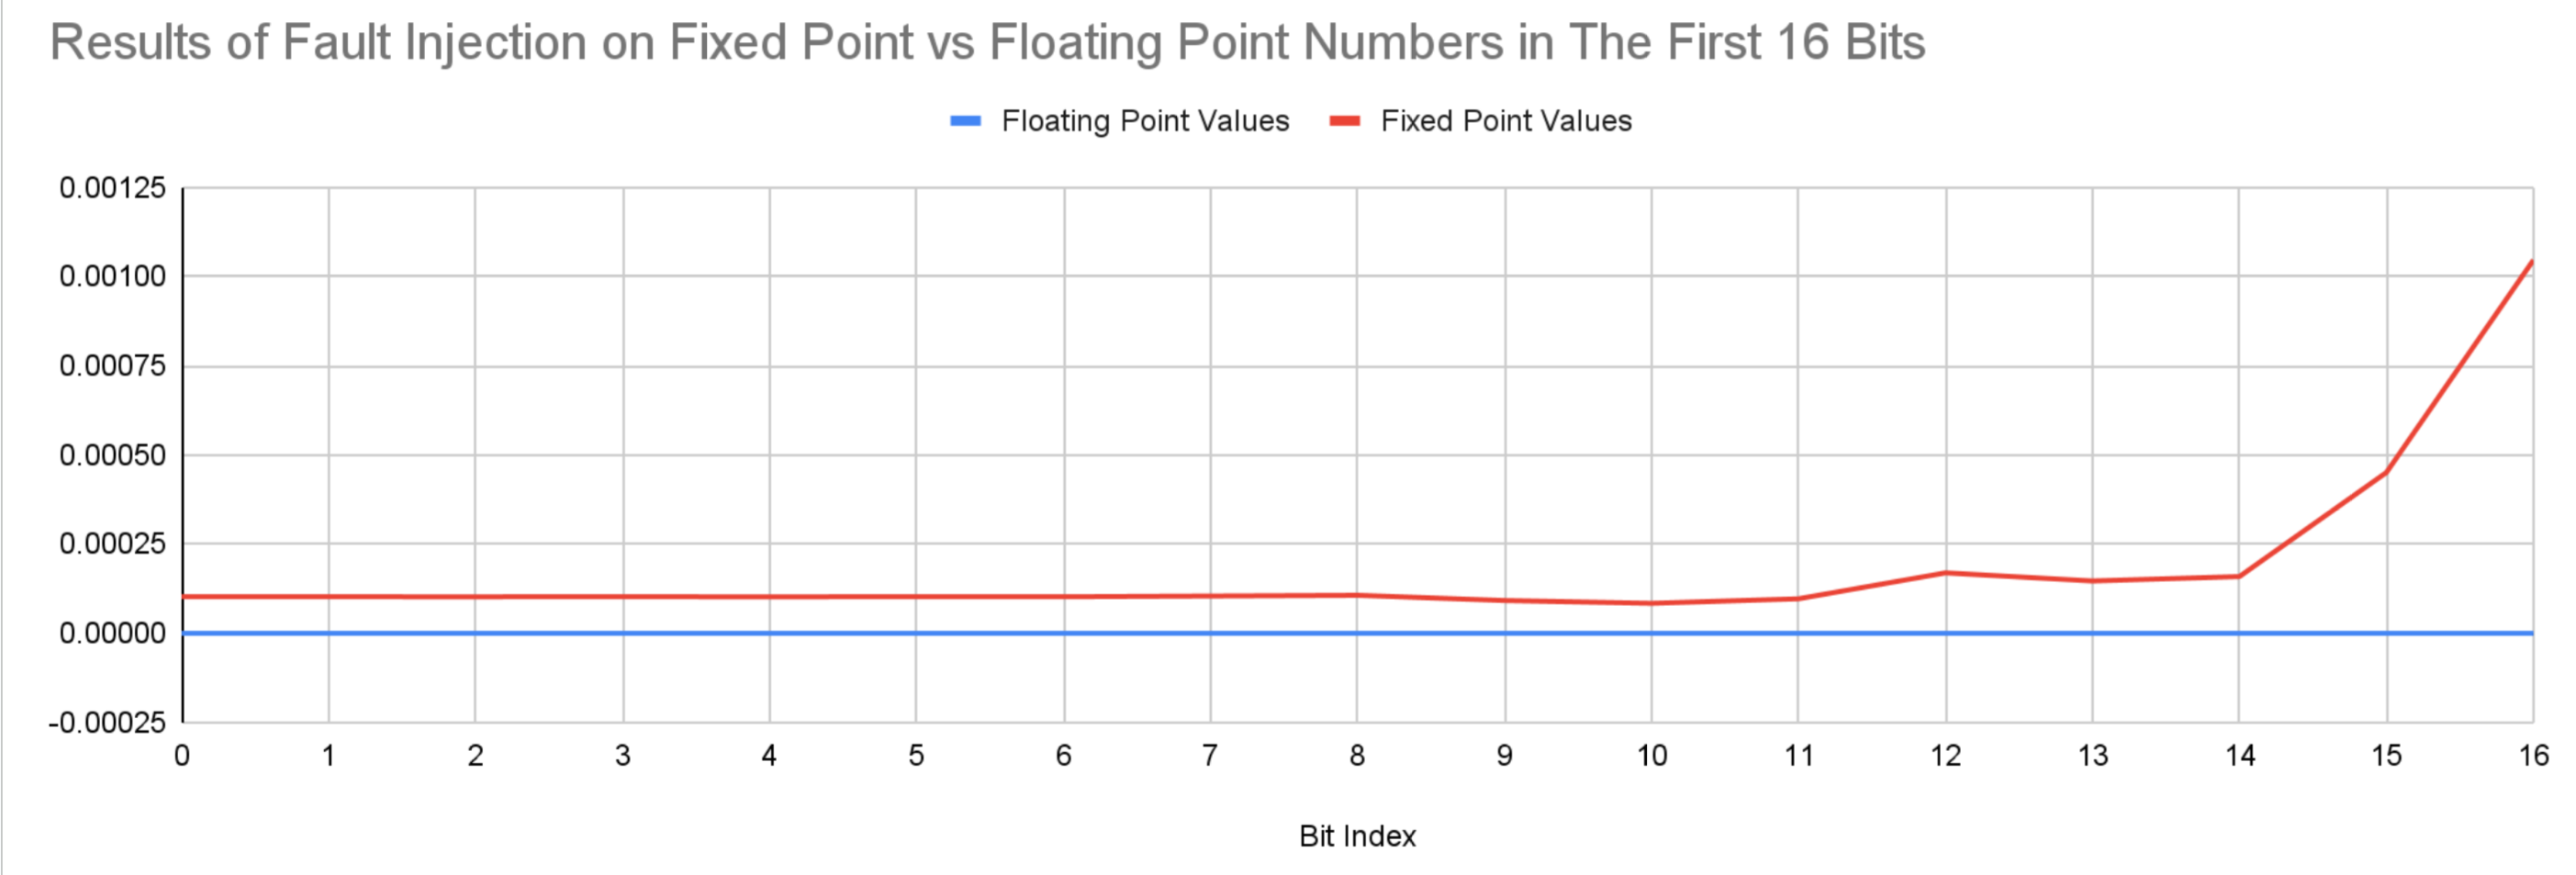
\includegraphics[width=0.5\linewidth]{graph_fault_injection_fix_vs_float_first_16_bits.png}
    \caption{The fixed point error is magnitudes larger than the floating point error at its lowest.}
    \label{fig:graph_fixed_vs_float_error_first_16}
\end{figure}

When assessing how the injected faults affect the program behavior, it is helpful to use the failure classifications found in~\citet{failure_class_with_respect_to_detection} for subtle incorrect and coarse incorrect service values. A service is the behavior of a system as percieved by an external observer. For a perfect observer, i.e. an observer that can accurately map a service output as either a correct or incorrect output. Humans are rarely perfect, which puts us in a different category of observers able to discern between three different states of service delivery: correct, coarse incorrect, and subtle incorrect.  Coarse incorrect are states that are certainly false, correct states are observably correct, and subtle incorrect states are difficult to discern as being incorrect or correct, though they are in reality the result of incorrect service. This means that a value could be percieved as correct while actually being the result of faulty service. This can counterintuitively be a bigger issue than a very large error, in that it can be more difficult to detect~\citep{hodge2004survey}.

This is why the domain matters when discussing reliability. In the result, until injecting a fault in the bit at index 37, the floating point error remains lower than that of the fixed point implementation with no faults injected. In the bit at index 55, the error becomes larger than the highest error recorded for the fixed point implementations, and the error keeps rising until injecting an error at the bit in index 63, which is the sign bit.

If we define the standard fixed point version error as the threshold for a coarse error, the majority of floating point variable bit flips do not constitute a fault. 

For this benchmark, the precision was set such as to allow the use of 32 bit integers for the fixed point implementation. This was done by the authors of taffo through the use of annotations specifying the range of values that the variables can contain. This may not be the case for all the benchmarks in the included polybench benchmark suite.

% discuss the error, how error rate changes with injected bit, implications taking subtle and coarse errors into account. Subtle errors may have a larger effect on scientific calculations or highly sensitive calculations such as for satellite navigation or space travel, where if travelling very long distances a small error may result in a huge deviation. Larger errors may be easier to discover.
A larger deviation may be easier to discover than a lower deviation, either through statistics or detection algorithms~\citep{hodge2004survey}. The fact that many bits in a 64-bit floating point number can be injected without a significant effect on the calculation may be an advantage if the calculation in question is fault tolerant at heart. Floating point errors go up very quickly when the error hits the exponent part of the number, so detecting a fault above a certain threshold is feasible.

On the other hand, while the smallest faults injected into fixed point numbers are larger than the smallest faults in floating point numbers, a number where only the 32 lowest bits will affect the calculations that follow have 32 bits where nothing happens when they are flipped. This is true given the assumption that only data bits are flipped, when this is not necessarily the case.

\subsection{Weaknesses in the Fault Injection Campaign}

The design of the fault injection campaign was influenced by the available approximate computing tools. Both tools works using the same principle, reducing precision for compatible computations, so seeing how injecting bits of different significance in reference data affect different internal bit representations/bit widths of numbers is of great interest for both tools. For a tool that does not perform any additional casting operations, this is less interesting, though not irrelevant. 

Designing a software fault injection campaign should involve reasoning about the code base: The faults injected should with preference reflect faults that may occur in production environments. This is important for both developmental faults and operational faults because biases in the injection of faults will lead to bias in the results of the fault injection. For instance, injecting developmental faults mainly in  well-tested sections of code may be less relevant than injecting developmental faults in parts of the code that have a lower degree of test coverage if the kind of fault that is injected is caught by the regression tests. 

This fault injection campaign only considers faults of one kind, namely bit flips in supplied data to the kernel. The bit flip are quite drastic as they are injected into every single variable supplied as data to the function. This does not necessarily realistically represent the faults that would occur in production, and gives a more extreme picture of the effect of fault injection on a program that approximates through converting variables to fixed point types. 

Given more time, implementing an approach as outlined in~\citep{van2016finding} would be preferable. \citep{van2016finding} maintains that a fault injection campaign requires a good fault model, that is an overview of the faults that may occur and in what frequency they occur, and to perform fault injections that follows this fault model. When a fault model does not correspond with the faults that are actually executed during the fault injection campaign either the fault model is lacking or the fault injection campaign has not gathered enough data. 

According to \citep{van2016finding} coverage has a significant impact on the fault injection results. Coverage here means the amount of code that is executed throughout the fault injection campaign. If an injected fault is not run throughout the campaign (the fault is not "activated"), the results of the fault injection will not represent the effect of this fault. In this campaign, all the faults injected above the bit in index 31 for the fixed point implementation falls in this category: The fault is truncated away, and is therefore not activated. 

All in all, the focus of the fault injection campaign ended up being on the benchmarks and the tools themselves, not on approximate computing, leading to results that say more about how the benchmark code behaves than the fault injection technique itself. This was due to time constraints caused by focusing too much on using tools that were supposed to simplify fault injection through quickly creating approximate versions of precise programs. Instead of spending time making the tools work, time would have been better spent using approximate computing techniques to manually create multiple versions of the same code, preferably within a domain that allows for clear definitions of both silent data corruptions and hard failures, such as a facial recognition application. The different versions of this approximate computing code would then have their own fault model that reflects the different quirks of the different techniques. 



\subsection{code quality}

On a different note, the code changes of the validation script result in a more understandable piece of software.

The comparison script written for the fault injection comparison is not perfect either. However, the assumptions are documented, and tests support and explain functionality. 
%This is difficult to realize when using python as a scripting language, but at the very least variable names need to be descriptive, and file outputs need to follow the existing standards and descriptions (for instance not mislabeling an output as a .csv file).

Some changes were apparent not because of the programming skills of the author, but simply because of an IDE tool highlighting errors that were easy to remedy. Figure~\ref{fig:IDE_highlighting} shows the highlighted error, which in this case is a keyword that does nothing. In this case the error is that the code describes functionality that is not possible.

\begin{figure}[h]
    \centering
    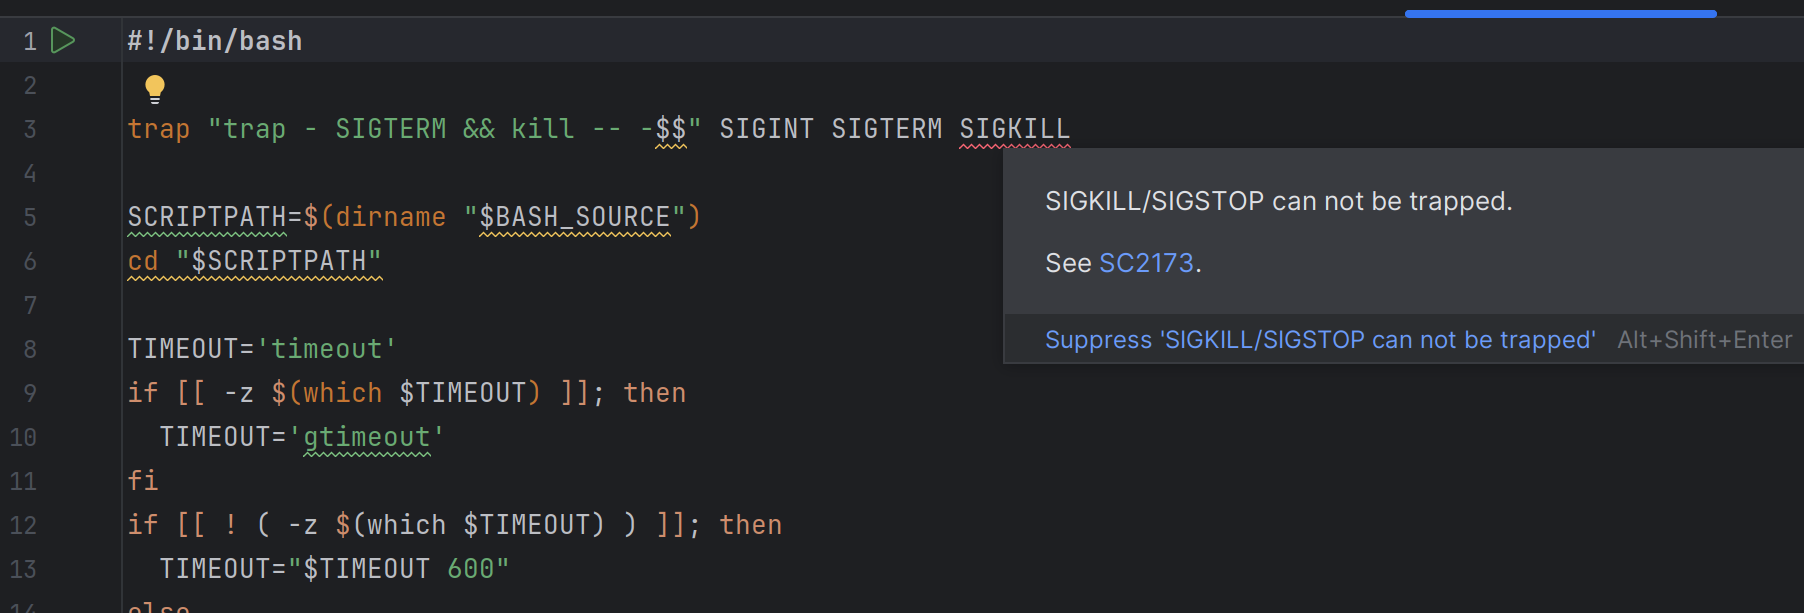
\includegraphics[width=0.5\linewidth]{Images/IDE_highlighting.png}
    \caption{the IDE, in this case CLion, highlighting an error in a shell script.}
    \label{fig:IDE_highlighting}
\end{figure}
% There is a habit of writing code as if to be archived forever. The documentation lags behind, and there is no test suite for the tool

There are many aspects of programming that can be measured to provide an indication of code quality. One such example is test coverage, which measures how many lines of the written code is executed through tests, and a higher percentage of code executed in tests is better. Although a program has 100\% code coverage, this alone does not designate the program as a good program: The tests themselves need to specify what behavior they test, and the test needs to assert that the output aligns with the expected output, such that if there is a change in the code that changes this behavior the test should fail. Quantitative code quality metrics are intended to be used as an aid in writing good code, not as designators of good or bad code. 

Using quantitative code quality metrics is a more reliable qualifier of bad code. Taking coverage again as the example metric, while a high coverage cannot be used alone to decide whether code is well written or not, a low coverage is a good indication of code that doesn't follow standard development practices.  


\subsection{Differences between documentation and implementation}

There are deviations in \taffo{} which are not documented in neither the code repository nor the papers published about \taffo{}. 
This includes facts such as the error propagator not doing what is described in the papers describing taffo, and the installation instructions of \taffo{} not being foolproof, at least not for the fool of a thesis author in question.

The error propagation pass of taffo is by default disabled on the polybench-cpu script that compiles, runs, and evaluates the benchmarks. When enabling it, it produces an estimated maximum error for a specified target in a file given a tranformation of the target from floating point to fixed point. This estimation does not correspond to and is in fact quite different from the actual result recorded in the bench-results directory. for instance, for the benchmark 2mm found in the directory linear-algebra/kernel/2mm, the output of the error propagator pass is shown in listing~\ref{listing:error_prop_2mm}.

\begin{lstlisting}
*** Target Errors: ***
Computed error for target D: 3.126388e-14
\end{lstlisting}
\caption{Output of the \taffo{} error propagator for the benchmark 2mm.}
\label{listing:error_prop_2mm}

This is quite a lot lower than the actual error recorded when running the fixed point implementation of the benchmark against the floating point implementation, which is 0.1438640358449807895808080808. See the table in appendix~\ref{appendix:vra_2mm} for the complete results for the complete 2mm benchmark results. This difference may be due to a misunderstanding of what the output actually tells us, but this too in itself is part of what has made this project challenging.

To enable debugging and further development of \taffo{}, the README specifies that a debug build of LLVM is required. Despite repeated attempts, there has only been one successful install of \taffo{} during the course of this project using a debug build of LLVM, and this successful build was not repeatable despite a clean OS install and following the exact same steps. This included making changes in the source code of a dependency within a \taffo{} dependency.  

Though there is both a test and a test-lit folder in the \taffo{} project neither is documented in the README or elsewhere, and the tests themselves are cryptic. This last fact may be due to the design of lit itself, which requires some knowledge of the framework to understand the tests. 

In addition to not being very declarative in the test descriptions, the tests folder contains a lot of benchmarks. These are not tests in that they do not assert some kind of functionality that can be verified, only whether the code produces \*some\* output. Therefore it should not reside in the tests folder, but perhaps a folder named benchmarks.

\taffo{}, when called using the parameters in the existing compile script, produces LLVM bytecode files. These files are numbered according to which optimisation pass they represent in the taffo compilation process. \taffo{} has a flag called emit-llvm that is supposed to emit LLVM bytecode, and does so, but this LLVM bytecode is not linked even though the taffo command specifies that it should, while also not producing any errors when compiling. To get llvm bytecode that is linked you need to either link it manually, or take the existing LLVM bytecode intermediate files. this was discovered through troubleshooting. 



\cleardoublepage

\chapter{Challenges}
%! Author = lars
%! Date = 6/22/25

The completion of this thesis has presented difficulties that has caused delays. The difficulties range from the difficulties that are to be expected of a masters thesis to issues that complicate the writing of this thesis unnecessarily. The following sections will present the biggest difficulties that this thesis presented. 


% \section{Availability of Approximate Computing Tools}




\section{Software}
Code quality is a concept that is difficult to quantify exactly.

It includes whether a program behaves as expected when running, but also properties of the program that cannot be seen during operation such as variable naming, code duplication and test coverage.
The development environment of the code is also a part of code quality, for instance whether the codebase is built using
continuous integration and continuous deployment.

% A trend (anectotal for now) in software produced in scientific studies, is that they do not generally follow established norms and rules for software development.
% This leads to code that is not easy to understand (for instance, using
% variable names such as x and y), code that is difficult to continue work on, and perhaps the most critical: code that
% does not run.
% Even worse than writing a paper on a new type of software that is not written using common coding practices, is not making the code that you have written a paper about available to the public.

% Multiple approximate computing tools described in papers found in the initial study for this thesis, such as green CITE and \ldots, were simply not available, to a degree invalidating the results in the study.

FlexFloat, another tool found in the study, allows users to manually modify the mantissa and exponent width of a floating point variable, and emulate these custom types on architectures that do not have them. The tool also allows users to investigate how the error propagates through the program, and choose a fitting custom floating point type. This program did not seem relevant, as it targets development of code for custom hardware in embedded applications.

\taffo{} is the tool that most of the efforts of this project has been focused on. \taffo{} is a tool that has been developed for a number of years, and runs as an add-on to the well-established clang compiler in the LLVM-project.
\taffo{} is the tuning assistant for floating point to fixed point optimisation. The tool consists of 5 passes: the initialization pass, value range analysis, data type allocation, code conversion and error propagation pass.

There is some debate in the developer community about where to document code: some say it is better to document code through the test suite and through descriptive variable naming and the like, while others claim that documentation should be located in separate files. There is a clear consensus though that no documentation is better than wrong documentation.
The documentation that follows in \taffo{} does not accurately reflect what the best practices are, and the paper that describes \taffo{} does not accurately reflect the current capabilities of the tool.

Building the tool was not intuitive when following the documentation in the repository, for instance the documentations recommends building a specific version of clang from source, and then building \taffo{} while bundling it with this version of clang. The instructions lack certain important factors, such as it being necessary to specify which system compiler to use when compiling \taffo , moreover while using a debug version of clang built from source does not work, it works when downloading pre-built binaries.
Furthermore, the error-propagation pass does not work any more. This makes it difficult to use this project for other experimental purposes.

% The documentation of the annotation syntax is lacking. There is no comprehensive list of what variable types that are supported (or not supported) by the tool, making usage of \taffo{} a betting game.
\cleardoublepage

\chapter{Conclusion}
\section{Conclusion}

There are tools that can produce program code with reduced precision that at first glance can boast similar levels of reliability as "vanilla" programs, programs that are produced/compiled using only generally available compilers such as Clang or GCC (for C programs at least). 
The code quality of existing tools make concluding for or against existing approximate computing tools difficult. 

Of the tools that are described in literature, only floatsmith and \taffo{} aim to improve processing speeds independent of hardware and have source code readily available. Floatsmith is not sufficiently tested with larger code repositories and would not work with the selected benchmark.\taffo{} behavior is not sufficiently documented in the code through tests and internal documentation, and there are no passing builds in the CI-setup on github at the time of writing, complicating the assessment of the tool.

The goal of the thesis was to develop knowledge of inherent reliability properties (or the lack thereof) within approximate computing. Approximate computing is a broad category that consists of many different strategies which often do not overlap. The category that was investigated in this thesis was approximate computing by reducing the precision of the intermediate calculations. Through a one bit-flip at a time fault injection campaign on an established CPU benchmark augmented to function with \taffo{}, the program behaves in a predictable manner conducive to reliability. This cannot be used to infer reliability properties of other approximate computing techniques because of how the approaches differ, and the lack of available source code for  tools that are proven to improve efficiency and/or speed of computer programs. 
\cleardoublepage

\chapter{Further Work}

The next campaign would be performed on non-benchmark code. The chosen library was OpenCV which is used for computer vision applications in python and C++, more specifically a facial recognition example written using the OpenCV library. The fault injection planned here would also be single bit fault injections in variables, however as the output from these functions are not numbers but a graphical representation of where a face in an image is, the error would be measured in how many frames, if at all, a face is detected in a standard video representation.

To collect data on developmental faults, i.e., faults that do not occur when the code is running but occur during the development of the code, another campaign was planned. This fault injection campaign was inspired by the technique and paper on G-SWFIT.


\cleardoublepage

\chapter{Sustainability Analysis}
\section{Sustainability analysis}
The motivation behind this thesis is rooted in sustainability. Enabling the usage of coding techniques that can reduce power consumption on existing hardware aligns well with sustainability goal number 9 of the UN sustainable development goals: 'Build resilient infrastructure, promote inclusive and sustainable industrialization and foster innovation'. 

The UN sustainability goals are a set of goals that the entirety of the UN have adopted. It is a common framework used by the member nations to make better choices with respect to the environment, both physical and social. The goals include gender and racial equality as well as reducing emissions from industry.

Just like approximate computing is a tradeoff between precision and processing speed/power consumption, implementing \emph{all} of the sustainability goals requires making some tradeoffs between the difference categories. 

All the categories represent unquestionable quality of life improvements for all humans, though enacting them may result in contraticting results. For instance, goal 1 is to end poverty in all its forms everywhere. So a factory gets established, which creates several jobs for the empoverished residents at this location. However, the factory produces runoff that contaminates a nearby water source, going against goal number 6 of ensuring availability and sustainability of water and sanitation for all. 

The following analysis has been created using a lightweight version of SusAF (Sustainability Assessment Framework)~\cite{SusAF_website}. SusAF divides sustainability effects into 5 categories: Social, individual, technical, economic and environmental. The social aspect describes how the artifact under review affects interpersonal relationships, and the individual aspect describe changes in personal health and quality of life. The technical aspect concerns itself with the lifecycle of a product or service, and how the service can be adapted to changing needs or technical demands. The economic aspect describes how the artifact under review changes the business side of things, whether performing research or creating monetary value becomes easier or harder. Finally, the Environmental aspect describe how the artifact under review may affect nature, through increasing or decreasing the load on nature through human presence.

The artifact under review for this thesis is an analysis of reliability in approximate computing tools. The intended audience consists of approximate computing system developers and system architects looking to improve efficiency of their solution, and the analysis will be performed from their point of view. 

\subsection{Individual Impacts}
Individual impacts of the analysis consists of 
\subsection{Social Impacts}

\subsection{Technical Impacts}


\cleardoublepage

\addcontentsline{toc}{chapter}{\protect\numberline{}References}
\bibliography{references}
% \printbibliography[title={References}] %you may change the title in the toc here if you want
\cleardoublepage

\appendix
%\chapter{\LARGE \textbf{Detailed Results}}
\chapter{Detailed Results}
\fancyhf{} %clear the header, it should be empty for the appendices
\renewcommand{\headrulewidth}{0pt} %no rule
\fancyfoot[C]{\thepage} %set the page numbers in the center of the footer instead 

%it is possible to set a different page numbering style for the appendix, but I personally just continued with the same page numbering as the main content as I find that more tidy
%\pagenumbering{roman}
%\setcounter{page}{1}
%\addcontentsline{toc}{chapter}{\protect\numberline{}Appendices:}

\section{Appendix}

\subsection{Complete results from fault injection}\label{appendix:complete_injection_results}
\begin{comment}
\begin{verbatim}[label=lst:injection_results]

Filename                        Average Difference From Control         Alternative Implementation Results
seidel-2d.float.txt             0.0                                     0.00010252590179347587
seidel-2d.txt                   0.00010252590179347587                  0.0
seidel-2d_bit_no_1.fixed.txt    0.00010252973353766834                  7.836499591601375e-15
seidel-2d_bit_no_1.float.txt    7.836499591601375e-15                   0.00010252973353766834
seidel-2d_bit_no_2.fixed.txt    0.00010242978918456464                  1.0070183402433041e-14
seidel-2d_bit_no_2.float.txt    1.0070183402433041e-14                  0.00010242978918456464
seidel-2d_bit_no_3.fixed.txt    0.00010269591987037501                  1.7122632695390493e-14
seidel-2d_bit_no_3.float.txt    1.7122632695390493e-14                  0.00010269591987037501
seidel-2d_bit_no_4.fixed.txt    0.00010227745091820854                  2.8727424627485174e-14
seidel-2d_bit_no_4.float.txt    2.8727424627485174e-14                  0.00010227745091820854
seidel-2d_bit_no_5.fixed.txt    0.00010277981877232038                  5.09567649902877e-14
seidel-2d_bit_no_5.float.txt    5.09567649902877e-14                    0.00010277981877232038
seidel-2d_bit_no_6.fixed.txt    0.00010250126707458161                  8.628055195216561e-14
seidel-2d_bit_no_6.float.txt    8.628055195216561e-14                   0.00010250126707458161
seidel-2d_bit_no_7.fixed.txt    0.00010450026309392104                  1.2886278998079994e-13
seidel-2d_bit_no_7.float.txt    1.2886278998079994e-13                  0.00010450026309392104
seidel-2d_bit_no_8.fixed.txt    0.00010662387752436846                  2.3631074870349154e-13
seidel-2d_bit_no_8.float.txt    2.3631074870349154e-13                  0.00010662387752436846
seidel-2d_bit_no_9.fixed.txt    9.194230723288186e-05                   4.625698030993539e-13
seidel-2d_bit_no_9.float.txt    4.625698030993539e-13                   9.194230723288186e-05
seidel-2d_bit_no_10.fixed.txt   8.414004397302073e-05                   7.814396866027106e-13
seidel-2d_bit_no_10.float.txt   7.814396866027106e-13                   8.414004397302073e-05
seidel-2d_bit_no_11.fixed.txt   9.683497321514389e-05                   1.949109275844671e-12
seidel-2d_bit_no_11.float.txt   1.949109275844671e-12                   9.683497321514389e-05
seidel-2d_bit_no_12.fixed.txt   0.00016945311659486383                  5.926170726735548e-12
seidel-2d_bit_no_12.float.txt   5.926170726735548e-12                   0.00016945311659486383
seidel-2d_bit_no_13.fixed.txt   0.00014676695716469516                  1.1517751583576575e-11
seidel-2d_bit_no_13.float.txt   1.1517751583576575e-11                  0.00014676695716469516
seidel-2d_bit_no_14.fixed.txt   0.00015912330669092686                  1.7147093324539844e-11
seidel-2d_bit_no_14.float.txt   1.7147093324539844e-11                  0.00015912330669092686
seidel-2d_bit_no_15.fixed.txt   0.0004508313725003589                   3.461998942767223e-11
seidel-2d_bit_no_15.float.txt   3.461998942767223e-11                   0.0004508313725003589
seidel-2d_bit_no_16.fixed.txt   0.0010460176076898182                   7.976829700127646e-11
seidel-2d_bit_no_16.float.txt   7.976829700127646e-11                   0.0010460176076898182
seidel-2d_bit_no_17.fixed.txt   0.0042558195475949955                   1.2204403410519433e-10
seidel-2d_bit_no_17.float.txt   1.2204403410519433e-10                  0.0042558195475949955
seidel-2d_bit_no_18.fixed.txt   0.0064681208001982834                   2.373641398611048e-10
seidel-2d_bit_no_18.float.txt   2.373641398611048e-10                   0.0064681208001982834
seidel-2d_bit_no_19.fixed.txt   0.010572742354750364                    6.776253971886386e-10
seidel-2d_bit_no_19.float.txt   6.776253971886386e-10                   0.010572742354750364
seidel-2d_bit_no_20.fixed.txt   0.022732906050977938                    1.6178958072901225e-09
seidel-2d_bit_no_20.float.txt   1.6178958072901225e-09                  0.022732906050977938
seidel-2d_bit_no_21.fixed.txt   0.04624822179096891                     2.900568751875029e-09
seidel-2d_bit_no_21.float.txt   2.900568751875029e-09                   0.04624822179096891
seidel-2d_bit_no_22.fixed.txt   0.05676147859394719                     4.463706821820652e-09
seidel-2d_bit_no_22.float.txt   4.463706821820652e-09                   0.05676147859394719
seidel-2d_bit_no_23.fixed.txt   0.11553374815410823                     7.041500121288634e-09
seidel-2d_bit_no_23.float.txt   7.041500121288634e-09                   0.11553374815410823
seidel-2d_bit_no_24.fixed.txt   0.2791558806105791                      1.5552431969620665e-08
seidel-2d_bit_no_24.float.txt   1.5552431969620665e-08                  0.2791558806105791
seidel-2d_bit_no_25.fixed.txt   0.9828830033440512                      3.7436499037469934e-08
seidel-2d_bit_no_25.float.txt   3.7436499037469934e-08                  0.9828830033440512
seidel-2d_bit_no_26.fixed.txt   5.123534709237707                       6.479593805265462e-08
seidel-2d_bit_no_26.float.txt   6.479593805265462e-08                   5.123534709237707
seidel-2d_bit_no_27.fixed.txt   20.34871134608706                       1.1086531044075003e-07
seidel-2d_bit_no_27.float.txt   1.1086531044075003e-07                  20.34871134608706
seidel-2d_bit_no_28.fixed.txt   53.444575446692376                      2.1492355299898596e-07
seidel-2d_bit_no_28.float.txt   2.1492355299898596e-07                  53.444575446692376
seidel-2d_bit_no_29.fixed.txt   118.06806922736634                      4.875080832471769e-07
seidel-2d_bit_no_29.float.txt   4.875080832471769e-07                   118.06806922736634
seidel-2d_bit_no_30.fixed.txt   240.38767306192983                      8.453350257722744e-07
seidel-2d_bit_no_30.float.txt   8.453350257722744e-07                   240.38767306192983
seidel-2d_bit_no_31.fixed.txt   432.92573090152945                      2.020661384195993e-06
seidel-2d_bit_no_31.float.txt   2.020661384195993e-06                   432.92573090152945
seidel-2d_bit_no_32.fixed.txt   0.00010252590179347587                  6.188653891382238e-06
seidel-2d_bit_no_32.float.txt   6.188653891382238e-06                   0.00010252590179347587
seidel-2d_bit_no_33.fixed.txt   0.00010252590179347587                  1.2067690542822415e-05
seidel-2d_bit_no_33.float.txt   1.2067690542822415e-05                  0.00010252590179347587
seidel-2d_bit_no_34.fixed.txt   0.00010252590179347587                  1.7975386379592478e-05
seidel-2d_bit_no_34.float.txt   1.7975386379592478e-05                  0.00010252590179347587
seidel-2d_bit_no_35.fixed.txt   0.00010252590179347587                  3.630068274298885e-05
seidel-2d_bit_no_35.float.txt   3.630068274298885e-05                   0.00010252590179347587
seidel-2d_bit_no_36.fixed.txt   0.00010252590179347587                  8.364188265808143e-05
seidel-2d_bit_no_36.float.txt   8.364188265808143e-05                   0.00010252590179347587
seidel-2d_bit_no_37.fixed.txt   0.00010252590179347587                  0.00012797032836168635
seidel-2d_bit_no_37.float.txt   0.00012797032836168635                  0.00010252590179347587
seidel-2d_bit_no_38.fixed.txt   0.00010252590179347587                  0.00024889467014402257
seidel-2d_bit_no_38.float.txt   0.00024889467014402257                  0.00010252590179347587
seidel-2d_bit_no_39.fixed.txt   0.00010252590179347587                  0.0007105416960589848
seidel-2d_bit_no_39.float.txt   0.0007105416960589848                   0.00010252590179347587
seidel-2d_bit_no_40.fixed.txt   0.00010252590179347587                  0.0019417624576080793
seidel-2d_bit_no_40.float.txt   0.0019417624576080793                   0.00010252590179347587
seidel-2d_bit_no_41.fixed.txt   0.00010252590179347587                  0.003943187647018381
seidel-2d_bit_no_41.float.txt   0.003943187647018381                    0.00010252590179347587
seidel-2d_bit_no_42.fixed.txt   0.00010252590179347587                  0.007150903672185747
seidel-2d_bit_no_42.float.txt   0.007150903672185747                    0.00010252590179347587
seidel-2d_bit_no_43.fixed.txt   0.00010252590179347587                  0.013355891583010197
seidel-2d_bit_no_43.float.txt   0.013355891583010197                    0.00010252590179347587
seidel-2d_bit_no_44.fixed.txt   0.00010252590179347587                  0.013081305310932996
seidel-2d_bit_no_44.float.txt   0.013081305310932996                    0.00010252590179347587
seidel-2d_bit_no_45.fixed.txt   0.00010252590179347587                  0.01797072542866801
seidel-2d_bit_no_45.float.txt   0.01797072542866801                     0.00010252590179347587
seidel-2d_bit_no_46.fixed.txt   0.00010252590179347587                  0.03683588086365033
seidel-2d_bit_no_46.float.txt   0.03683588086365033                     0.00010252590179347587
seidel-2d_bit_no_47.fixed.txt   0.00010252590179347587                  0.1075653417011947
seidel-2d_bit_no_47.float.txt   0.1075653417011947                      0.00010252590179347587
seidel-2d_bit_no_48.fixed.txt   0.00010252590179347587                  0.38882888088824635
seidel-2d_bit_no_48.float.txt   0.38882888088824635                     0.00010252590179347587
seidel-2d_bit_no_49.fixed.txt   0.00010252590179347587                  1.9890269298258314
seidel-2d_bit_no_49.float.txt   1.9890269298258314                      0.00010252590179347587
seidel-2d_bit_no_50.fixed.txt   0.00010252590179347587                  8.629012699261413
seidel-2d_bit_no_50.float.txt   8.629012699261413                       0.00010252590179347587
seidel-2d_bit_no_51.fixed.txt   0.00010252590179347587                  25.795382086159993
seidel-2d_bit_no_51.float.txt   25.795382086159993                      0.00010252590179347587
seidel-2d_bit_no_52.fixed.txt   0.00010252590179347587                  64.65331813450862
seidel-2d_bit_no_52.float.txt   64.65331813450862                       0.00010252590179347587
seidel-2d_bit_no_53.fixed.txt   0.00010252590179347587                  132.3054843277936
seidel-2d_bit_no_53.float.txt   132.3054843277936                       0.00010252590179347587
seidel-2d_bit_no_54.fixed.txt   0.00010252590179347587                  140.41412113413136
seidel-2d_bit_no_54.float.txt   140.41412113413136                      0.00010252590179347587
seidel-2d_bit_no_55.fixed.txt   0.00010252590179347587                  25619.825047812476
seidel-2d_bit_no_55.float.txt   25619.825047812476                      0.00010252590179347587
seidel-2d_bit_no_56.fixed.txt   0.00010252590179347587                  6584294.581178659
seidel-2d_bit_no_56.float.txt   6584294.581178659                       0.00010252590179347587
seidel-2d_bit_no_57.fixed.txt   0.00010252590179347587                  431514915814.9726
seidel-2d_bit_no_57.float.txt   431514915814.9726                       0.00010252590179347587
seidel-2d_bit_no_58.fixed.txt   0.00010252590179347587                  1.8533424515933319e+21
seidel-2d_bit_no_58.float.txt   1.8533424515933319e+21                  0.00010252590179347587
seidel-2d_bit_no_59.fixed.txt   0.00010252590179347587                  3.4188133885483626e+40
seidel-2d_bit_no_59.float.txt   3.4188133885483626e+40                  0.00010252590179347587
seidel-2d_bit_no_60.fixed.txt   0.00010252590179347587                  1.1633619119162309e+79
seidel-2d_bit_no_60.float.txt   1.1633619119162309e+79                  0.00010252590179347587
seidel-2d_bit_no_61.fixed.txt   0.00010252590179347587                  1.3470810631989899e+156
seidel-2d_bit_no_61.float.txt   1.3470810631989899e+156                 0.00010252590179347587
seidel-2d_bit_no_62.fixed.txt   0.00010252590179347587                  nan
seidel-2d_bit_no_62.float.txt   nan                                     0.00010252590179347587
seidel-2d_bit_no_63.fixed.txt   0.00010252590179347587                  201.00625000002313
seidel-2d_bit_no_63.float.txt   201.00625000002313                      0.00010252590179347587
seidel-2d_bit_no_64.fixed.txt   100.26608126362525                      nan
seidel-2d_bit_no_64.float.txt   nan                                     100.26608126362525
seidel-2d_bit_no_65.fixed.txt   101.22680332254677                      nan
seidel-2d_bit_no_65.float.txt   nan                                     101.22680332254677
seidel-2d_bit_no_66.fixed.txt   99.22911101286253                       nan
seidel-2d_bit_no_66.float.txt   nan                                     99.22911101286253
seidel-2d_bit_no_70.fixed.txt   101.53423877332334                      nan
seidel-2d_bit_no_70.float.txt   nan                                     101.53423877332334
seidel-2d_bit_no_100.fixed.txt  99.39829564810347                       nan
seidel-2d_bit_no_100.float.txt  nan                                     99.39829564810347
\end{verbatim}
\end{comment}
% Table generated by Excel2LaTeX from sheet 'Sheet1'
\begin{longtable}{lll}
\caption{Injection results}
\label{lst:injection_results}\\
{\bf Filename} & {\bf Average Difference} & {\bf Alternative } \\
             & {\bf From Control }      & {\bf Implementation Results}\\
 
    seidel-2d.float.txt & 0.0   & 0.00010252590179347587 \\
    seidel-2d.txt & 0.00010252590179347587 & 0.0 \\
    seidel-2d\_bit\_no\_1.fixed.txt & 0.00010252973353766834 & 7.836499591601375e-15 \\
    seidel-2d\_bit\_no\_1.float.txt & 7.836499591601375e-15 & 0.00010252973353766834 \\
    seidel-2d\_bit\_no\_2.fixed.txt & 0.00010242978918456464 & 1.0070183402433041e-14 \\
    seidel-2d\_bit\_no\_2.float.txt & 1.0070183402433041e-14 & 0.00010242978918456464 \\
    seidel-2d\_bit\_no\_3.fixed.txt & 0.00010269591987037501 & 1.7122632695390493e-14 \\
    seidel-2d\_bit\_no\_3.float.txt & 1.7122632695390493e-14 & 0.00010269591987037501 \\
    seidel-2d\_bit\_no\_4.fixed.txt & 0.00010227745091820854 & 2.8727424627485174e-14 \\
    seidel-2d\_bit\_no\_4.float.txt & 2.8727424627485174e-14 & 0.00010227745091820854 \\
    seidel-2d\_bit\_no\_5.fixed.txt & 0.00010277981877232038 & 5.09567649902877e-14 \\
    seidel-2d\_bit\_no\_5.float.txt & 5.09567649902877e-14 & 0.00010277981877232038 \\
    seidel-2d\_bit\_no\_6.fixed.txt & 0.00010250126707458161 & 8.628055195216561e-14 \\
    seidel-2d\_bit\_no\_6.float.txt & 8.628055195216561e-14 & 0.00010250126707458161 \\
    seidel-2d\_bit\_no\_7.fixed.txt & 0.00010450026309392104 & 1.2886278998079994e-13 \\
    seidel-2d\_bit\_no\_7.float.txt & 1.2886278998079994e-13 & 0.00010450026309392104 \\
    seidel-2d\_bit\_no\_8.fixed.txt & 0.00010662387752436846 & 2.3631074870349154e-13 \\
    seidel-2d\_bit\_no\_8.float.txt & 2.3631074870349154e-13 & 0.00010662387752436846 \\
    seidel-2d\_bit\_no\_9.fixed.txt & 9.194230723288186e-05 & 4.625698030993539e-13 \\
    seidel-2d\_bit\_no\_9.float.txt & 4.625698030993539e-13 & 9.194230723288186e-05 \\
    seidel-2d\_bit\_no\_10.fixed.txt & 8.414004397302073e-05 & 7.814396866027106e-13 \\
    seidel-2d\_bit\_no\_10.float.txt & 7.814396866027106e-13 & 8.414004397302073e-05 \\
    seidel-2d\_bit\_no\_11.fixed.txt & 9.683497321514389e-05 & 1.949109275844671e-12 \\
    seidel-2d\_bit\_no\_11.float.txt & 1.949109275844671e-12 & 9.683497321514389e-05 \\
    seidel-2d\_bit\_no\_12.fixed.txt & 0.00016945311659486383 & 5.926170726735548e-12 \\
    seidel-2d\_bit\_no\_12.float.txt & 5.926170726735548e-12 & 0.00016945311659486383 \\
    seidel-2d\_bit\_no\_13.fixed.txt & 0.00014676695716469516 & 1.1517751583576575e-11 \\
    seidel-2d\_bit\_no\_13.float.txt & 1.1517751583576575e-11 & 0.00014676695716469516 \\
    seidel-2d\_bit\_no\_14.fixed.txt & 0.00015912330669092686 & 1.7147093324539844e-11 \\
    seidel-2d\_bit\_no\_14.float.txt & 1.7147093324539844e-11 & 0.00015912330669092686 \\
    seidel-2d\_bit\_no\_15.fixed.txt & 0.0004508313725003589 & 3.461998942767223e-11 \\
    seidel-2d\_bit\_no\_15.float.txt & 3.461998942767223e-11 & 0.0004508313725003589 \\
    seidel-2d\_bit\_no\_16.fixed.txt & 0.0010460176076898182 & 7.976829700127646e-11 \\
    seidel-2d\_bit\_no\_16.float.txt & 7.976829700127646e-11 & 0.0010460176076898182 \\
    seidel-2d\_bit\_no\_17.fixed.txt & 0.0042558195475949955 & 1.2204403410519433e-10 \\
    seidel-2d\_bit\_no\_17.float.txt & 1.2204403410519433e-10 & 0.0042558195475949955 \\
    seidel-2d\_bit\_no\_18.fixed.txt & 0.0064681208001982834 & 2.373641398611048e-10 \\
    seidel-2d\_bit\_no\_18.float.txt & 2.373641398611048e-10 & 0.0064681208001982834 \\
    seidel-2d\_bit\_no\_19.fixed.txt & 0.010572742354750364 & 6.776253971886386e-10 \\
    seidel-2d\_bit\_no\_19.float.txt & 6.776253971886386e-10 & 0.010572742354750364 \\
    seidel-2d\_bit\_no\_20.fixed.txt & 0.022732906050977938 & 1.6178958072901225e-09 \\
    seidel-2d\_bit\_no\_20.float.txt & 1.6178958072901225e-09 & 0.022732906050977938 \\
    seidel-2d\_bit\_no\_21.fixed.txt & 0.04624822179096891 & 2.900568751875029e-09 \\
    seidel-2d\_bit\_no\_21.float.txt & 2.900568751875029e-09 & 0.04624822179096891 \\
    seidel-2d\_bit\_no\_22.fixed.txt & 0.05676147859394719 & 4.463706821820652e-09 \\
    seidel-2d\_bit\_no\_22.float.txt & 4.463706821820652e-09 & 0.05676147859394719 \\
    seidel-2d\_bit\_no\_23.fixed.txt & 0.11553374815410823 & 7.041500121288634e-09 \\
    seidel-2d\_bit\_no\_23.float.txt & 7.041500121288634e-09 & 0.11553374815410823 \\
    seidel-2d\_bit\_no\_24.fixed.txt & 0.2791558806105791 & 1.5552431969620665e-08 \\
    seidel-2d\_bit\_no\_24.float.txt & 1.5552431969620665e-08 & 0.2791558806105791 \\
    seidel-2d\_bit\_no\_25.fixed.txt & 0.9828830033440512 & 3.7436499037469934e-08 \\
    seidel-2d\_bit\_no\_25.float.txt & 3.7436499037469934e-08 & 0.9828830033440512 \\
    seidel-2d\_bit\_no\_26.fixed.txt & 5.123534709237707 & 6.479593805265462e-08 \\
    seidel-2d\_bit\_no\_26.float.txt & 6.479593805265462e-08 & 5.123534709237707 \\
    seidel-2d\_bit\_no\_27.fixed.txt & 20.34871134608706 & 1.1086531044075003e-07 \\
    seidel-2d\_bit\_no\_27.float.txt & 1.1086531044075003e-07 & 20.34871134608706 \\
    seidel-2d\_bit\_no\_28.fixed.txt & 53.444575446692376 & 2.1492355299898596e-07 \\
    seidel-2d\_bit\_no\_28.float.txt & 2.1492355299898596e-07 & 53.444575446692376 \\
    seidel-2d\_bit\_no\_29.fixed.txt & 118.06806922736634 & 4.875080832471769e-07 \\
    seidel-2d\_bit\_no\_29.float.txt & 4.875080832471769e-07 & 118.06806922736634 \\
    seidel-2d\_bit\_no\_30.fixed.txt & 240.38767306192983 & 8.453350257722744e-07 \\
    seidel-2d\_bit\_no\_30.float.txt & 8.453350257722744e-07 & 240.38767306192983 \\
    seidel-2d\_bit\_no\_31.fixed.txt & 432.92573090152945 & 2.020661384195993e-06 \\
    seidel-2d\_bit\_no\_31.float.txt & 2.020661384195993e-06 & 432.92573090152945 \\
    seidel-2d\_bit\_no\_32.fixed.txt & 0.00010252590179347587 & 6.188653891382238e-06 \\
    seidel-2d\_bit\_no\_32.float.txt & 6.188653891382238e-06 & 0.00010252590179347587 \\
    seidel-2d\_bit\_no\_33.fixed.txt & 0.00010252590179347587 & 1.2067690542822415e-05 \\
    seidel-2d\_bit\_no\_33.float.txt & 1.2067690542822415e-05 & 0.00010252590179347587 \\
    seidel-2d\_bit\_no\_34.fixed.txt & 0.00010252590179347587 & 1.7975386379592478e-05 \\
    seidel-2d\_bit\_no\_34.float.txt & 1.7975386379592478e-05 & 0.00010252590179347587 \\
    seidel-2d\_bit\_no\_35.fixed.txt & 0.00010252590179347587 & 3.630068274298885e-05 \\
    seidel-2d\_bit\_no\_35.float.txt & 3.630068274298885e-05 & 0.00010252590179347587 \\
    seidel-2d\_bit\_no\_36.fixed.txt & 0.00010252590179347587 & 8.364188265808143e-05 \\
    seidel-2d\_bit\_no\_36.float.txt & 8.364188265808143e-05 & 0.00010252590179347587 \\
    seidel-2d\_bit\_no\_37.fixed.txt & 0.00010252590179347587 & 0.00012797032836168635 \\
    seidel-2d\_bit\_no\_37.float.txt & 0.00012797032836168635 & 0.00010252590179347587 \\
    seidel-2d\_bit\_no\_38.fixed.txt & 0.00010252590179347587 & 0.00024889467014402257 \\
    seidel-2d\_bit\_no\_38.float.txt & 0.00024889467014402257 & 0.00010252590179347587 \\
    seidel-2d\_bit\_no\_39.fixed.txt & 0.00010252590179347587 & 0.0007105416960589848 \\
    seidel-2d\_bit\_no\_39.float.txt & 0.0007105416960589848 & 0.00010252590179347587 \\
    seidel-2d\_bit\_no\_40.fixed.txt & 0.00010252590179347587 & 0.0019417624576080793 \\
    seidel-2d\_bit\_no\_40.float.txt & 0.0019417624576080793 & 0.00010252590179347587 \\
    seidel-2d\_bit\_no\_41.fixed.txt & 0.00010252590179347587 & 0.003943187647018381 \\
    seidel-2d\_bit\_no\_41.float.txt & 0.003943187647018381 & 0.00010252590179347587 \\
    seidel-2d\_bit\_no\_42.fixed.txt & 0.00010252590179347587 & 0.007150903672185747 \\
    seidel-2d\_bit\_no\_42.float.txt & 0.007150903672185747 & 0.00010252590179347587 \\
    seidel-2d\_bit\_no\_43.fixed.txt & 0.00010252590179347587 & 0.013355891583010197 \\
    seidel-2d\_bit\_no\_43.float.txt & 0.013355891583010197 & 0.00010252590179347587 \\
    seidel-2d\_bit\_no\_44.fixed.txt & 0.00010252590179347587 & 0.013081305310932996 \\
    seidel-2d\_bit\_no\_44.float.txt & 0.013081305310932996 & 0.00010252590179347587 \\
    seidel-2d\_bit\_no\_45.fixed.txt & 0.00010252590179347587 & 0.01797072542866801 \\
    seidel-2d\_bit\_no\_45.float.txt & 0.01797072542866801 & 0.00010252590179347587 \\
    seidel-2d\_bit\_no\_46.fixed.txt & 0.00010252590179347587 & 0.03683588086365033 \\
    seidel-2d\_bit\_no\_46.float.txt & 0.03683588086365033 & 0.00010252590179347587 \\
    seidel-2d\_bit\_no\_47.fixed.txt & 0.00010252590179347587 & 0.1075653417011947 \\
    seidel-2d\_bit\_no\_47.float.txt & 0.1075653417011947 & 0.00010252590179347587 \\
    seidel-2d\_bit\_no\_48.fixed.txt & 0.00010252590179347587 & 0.38882888088824635 \\
    seidel-2d\_bit\_no\_48.float.txt & 0.38882888088824635 & 0.00010252590179347587 \\
    seidel-2d\_bit\_no\_49.fixed.txt & 0.00010252590179347587 & 1.9890269298258314 \\
    seidel-2d\_bit\_no\_49.float.txt & 1.9890269298258314 & 0.00010252590179347587 \\
    seidel-2d\_bit\_no\_50.fixed.txt & 0.00010252590179347587 & 8.629012699261413 \\
    seidel-2d\_bit\_no\_50.float.txt & 8.629012699261413 & 0.00010252590179347587 \\
    seidel-2d\_bit\_no\_51.fixed.txt & 0.00010252590179347587 & 25.795382086159993 \\
    seidel-2d\_bit\_no\_51.float.txt & 25.795382086159993 & 0.00010252590179347587 \\
    seidel-2d\_bit\_no\_52.fixed.txt & 0.00010252590179347587 & 64.65331813450862 \\
    seidel-2d\_bit\_no\_52.float.txt & 64.65331813450862 & 0.00010252590179347587 \\
    seidel-2d\_bit\_no\_53.fixed.txt & 0.00010252590179347587 & 132.3054843277936 \\
    seidel-2d\_bit\_no\_53.float.txt & 132.3054843277936 & 0.00010252590179347587 \\
    seidel-2d\_bit\_no\_54.fixed.txt & 0.00010252590179347587 & 140.41412113413136 \\
    seidel-2d\_bit\_no\_54.float.txt & 140.41412113413136 & 0.00010252590179347587 \\
    seidel-2d\_bit\_no\_55.fixed.txt & 0.00010252590179347587 & 25619.825047812476 \\
    seidel-2d\_bit\_no\_55.float.txt & 25619.825047812476 & 0.00010252590179347587 \\
    seidel-2d\_bit\_no\_56.fixed.txt & 0.00010252590179347587 & 6584294.581178659 \\
    seidel-2d\_bit\_no\_56.float.txt & 6584294.581178659 & 0.00010252590179347587 \\
    seidel-2d\_bit\_no\_57.fixed.txt & 0.00010252590179347587 & 431514915814.9726 \\
    seidel-2d\_bit\_no\_57.float.txt & 431514915814.9726 & 0.00010252590179347587 \\
    seidel-2d\_bit\_no\_58.fixed.txt & 0.00010252590179347587 & 1.8533424515933319e+21 \\
    seidel-2d\_bit\_no\_58.float.txt & 1.8533424515933319e+21 & 0.00010252590179347587 \\
    seidel-2d\_bit\_no\_59.fixed.txt & 0.00010252590179347587 & 3.4188133885483626e+40 \\
    seidel-2d\_bit\_no\_59.float.txt & 3.4188133885483626e+40 & 0.00010252590179347587 \\
    seidel-2d\_bit\_no\_60.fixed.txt & 0.00010252590179347587 & 1.1633619119162309e+79 \\
    seidel-2d\_bit\_no\_60.float.txt & 1.1633619119162309e+79 & 0.00010252590179347587 \\
    seidel-2d\_bit\_no\_61.fixed.txt & 0.00010252590179347587 & 1.3470810631989899e+156 \\
    seidel-2d\_bit\_no\_61.float.txt & 1.3470810631989899e+156 & 0.00010252590179347587 \\
    seidel-2d\_bit\_no\_62.fixed.txt & 0.00010252590179347587 & nan \\
    seidel-2d\_bit\_no\_62.float.txt & nan   & 0.00010252590179347587 \\
    seidel-2d\_bit\_no\_63.fixed.txt & 0.00010252590179347587 & 201.00625000002313 \\
    seidel-2d\_bit\_no\_63.float.txt & 201.00625000002313 & 0.00010252590179347587 \\
    seidel-2d\_bit\_no\_64.fixed.txt & 100.26608126362525 & nan \\
    seidel-2d\_bit\_no\_64.float.txt & nan   & 100.26608126362525 \\
    seidel-2d\_bit\_no\_65.fixed.txt & 101.22680332254677 & nan \\
    seidel-2d\_bit\_no\_65.float.txt & nan   & 101.22680332254677 \\
    seidel-2d\_bit\_no\_66.fixed.txt & 99.22911101286253 & nan \\
    seidel-2d\_bit\_no\_66.float.txt & nan   & 99.22911101286253 \\
    seidel-2d\_bit\_no\_70.fixed.txt & 101.53423877332334 & nan \\
    seidel-2d\_bit\_no\_70.float.txt & nan   & 101.53423877332334 \\
    seidel-2d\_bit\_no\_100.fixed.txt & 99.39829564810347 & nan \\
    seidel-2d\_bit\_no\_100.float.txt & nan   & 99.39829564810347 \\
%\end{tabular}%
%  \label{tab:addlabel}%
\end{longtable}%



\end{document}
